\documentclass[11pt,a4paper]{article}
\usepackage[utf8]{inputenc}
\usepackage[T1]{fontenc}
\usepackage{mathpazo}
\usepackage{amsmath,amssymb}
\usepackage[a4paper,margin=2.4cm]{geometry}
\usepackage{graphicx}
\usepackage{pdflscape}
\usepackage{booktabs,array,longtable,tabularx}
\usepackage{xcolor}
\usepackage[numbers,square,sort&compress]{natbib}
\usepackage[most]{tcolorbox}
\usepackage{caption}
\usepackage{enumitem}
\usepackage{fancyhdr}
\usepackage{microtype}
\usepackage[colorlinks=true,linkcolor=bleu!70!black,citecolor=bleu!70!black,urlcolor=bleu!70!black]{hyperref}

\graphicspath{{./}{figures/}}
\definecolor{bleu}{HTML}{2A78D6}
\definecolor{orange}{HTML}{EB6834}
\definecolor{vert}{HTML}{139062}
\definecolor{gris}{HTML}{52514E}

% macros pour la bibliographie (BibTeX de l'auteur)
\newcommand{\apj}{Astrophys. J.}
\newcommand{\apjl}{Astrophys. J. Lett.}
\newcommand{\aj}{Astron. J.}

% unités et symboles
\newcommand{\Rt}{\ensuremath{R_\oplus}}
\newcommand{\Mt}{\ensuremath{M_\oplus}}
\newcommand{\ML}{\ensuremath{M_L}}
\newcommand{\LEM}{\ensuremath{L_{\rm EM}}}
\newcommand{\Req}{\ensuremath{R_{\rm eq}}}
\newcommand{\qB}{\ensuremath{q_B}}
\newcommand{\wt}{\ensuremath{\tilde\omega}}

% statuts
\newcommand{\stCalc}{\textcolor{vert}{\textbf{Calculé}}}
\newcommand{\stSup}{\textcolor{orange}{\textbf{Supposé}}}
\newcommand{\stOuv}{\textcolor{gris}{\textbf{Ouvert}}}
\newcommand{\stNon}{\textcolor{red!70!black}{\textbf{Non satisfait}}}

% encadrés
\newtcolorbox{simple}{enhanced,breakable,colback=bleu!5,colframe=bleu!70!black,boxrule=0.5pt,arc=2pt,left=7pt,right=7pt,top=4pt,bottom=4pt,fonttitle=\bfseries\small,title={En termes simples}}
\newtcolorbox{encadre}[1]{enhanced,breakable,colback=orange!6,colframe=orange!85!black,boxrule=0.5pt,arc=2pt,left=7pt,right=7pt,top=4pt,bottom=4pt,fonttitle=\bfseries\small,title={#1}}

\captionsetup{font=small,labelfont=bf,labelsep=period,width=0.94\linewidth}
\renewcommand{\figurename}{Figure}
\renewcommand{\tablename}{Tableau}
\renewcommand{\contentsname}{Table des matières}
\renewcommand{\refname}{Références}
\renewcommand{\bibsection}{\section*{Références}\addcontentsline{toc}{section}{Références}}
\renewcommand{\appendixname}{Annexe}
\setlength{\parskip}{4pt}
\setlength{\parindent}{0pt}
\renewcommand{\arraystretch}{1.12}
\setcounter{tocdepth}{2}

\pagestyle{fancy}
\fancyhf{}
\fancyhead[L]{\small M. Debailleul --- Théorie rétrodictive de l'origine de la Lune}
\fancyhead[R]{\small\thepage}
\fancyfoot[C]{\footnotesize \copyright{} 2026 Michel Debailleul --- Licence CC BY 4.0 --- ORCID 0009-0003-1222-1433}
\renewcommand{\headrulewidth}{0.3pt}

\hypersetup{pdftitle={Théorie rétrodictive de l'origine de la Lune : un disque secondaire circumterrestre redistribué par le survol rétrograde d'une planète rocheuse},pdfauthor={Michel Debailleul},pdfsubject={Origine de la Lune},pdfkeywords={origine de la Lune, disque secondaire, limite de Roche, survol rétrograde, marées}}

% guillemets français
\newcommand{\og}{«\nobreakspace\ignorespaces}
\newcommand{\fg}{\unskip\nobreakspace»}

\begin{document}

\thispagestyle{empty}
\begin{center}
{\LARGE\bfseries Théorie rétrodictive de l'origine de la Lune~:\\[4pt]
un disque secondaire circumterrestre redistribué\\[4pt]
par le survol rétrograde d'une planète rocheuse\par}
\vspace{16pt}
{\large\bfseries Michel Debailleul\par}
\vspace{3pt}
Géophysicien\\
Master~: Université libre de Bruxelles (ULB)\\
Chercheur indépendant\\
ORCID~: \href{https://orcid.org/0009-0003-1222-1433}{0009-0003-1222-1433}\\
\href{mailto:michel.debailleul@yahoo.fr}{michel.debailleul@yahoo.fr}\par
\vspace{6pt}
Octobre 2026\par
\smallskip DOI~: \href{https://doi.org/10.5281/zenodo.23391968}{10.5281/zenodo.23391968}\par
\end{center}
\vspace{4pt}

\begin{encadre}{Résumé}
\small
La Lune est une donnée, et la question est rétrodictive~: quels chemins physiques y conduisent, sans impact géant~? Le chemin examiné part d'une proto-Terre jeune et chaude, \emph{molle mais jamais liquide}, aplatie et gonflée par une rotation de $6$~h, entourée d'un disque de matière qui n'a pas encore formé de satellite. Une seconde planète rocheuse, la planète~$B$, passe près de la Terre à contresens de sa rotation, sans la toucher et sans lui donner de matière~: elle ne fait que tirer par gravitation. Elle remanie le disque (environ $47\,\%$ restent liés à la Terre, soit $3{,}5$ fois plus qu'avec un passage dans le sens de la rotation), fait basculer l'axe de la Terre et emporte un peu du moment cinétique de sa rotation. La matière restée liée s'assemble en un corps d'environ une masse lunaire dans chaque réalisation calculée~; il est conservé dans quatre réalisations sur dix, quand son orbite se fixe au-delà du rayon de corotation, et les marées le portent à la distance lunaire actuelle en $4{,}5$ milliards d'années.

\smallskip
\textbf{La correspondance isotopique.} Comme la planète~$B$ ne fournit aucune matière, la Lune est faite de matière terrestre~: l'identité isotopique Terre--Lune (O, Ti, Cr, $^{182}$W) et les déficits en V, Cr, Mn sont attendus d'emblée, là où l'impact géant doit les expliquer après coup.

\smallskip
\textbf{Le moment cinétique.} Le système lié contient $0{,}21\,\LEM$ de plus que le couple Terre--Lune actuel. Le freinage par la planète~$B$, la marée solaire et la résonance d'évection n'en retirent chacun qu'une part~; calculés ensemble sur une même trajectoire, ils ferment le bilan à $\pm0{,}05\,\LEM$ dans environ un quart à un tiers des trajectoires explorées, et à $\pm0{,}08\,\LEM$ dans environ deux cinquièmes à deux tiers, à deux conditions que le texte énonce~: une marée terrestre faible au début de l'histoire, comme il convient à un corps mou, et une contraction lente de la proto-Terre. Ces pourcentages décrivent la grille de paramètres étudiée, non une probabilité.

\smallskip
Les résultats sont des conditions nécessaires ou des familles de solutions, non des faits~; les limites sont dites section par section.

\smallskip
\textbf{Mots-clés.} origine de la Lune~; disque secondaire~; limite de Roche~; survol rétrograde~; corps mou~; marées~; évection~; rétrodiction.
\end{encadre}

\newpage
\tableofcontents
\newpage

% =====================================================================
\section{Le principe : lire l'origine de la Lune à rebours}
\label{sec:principe}

\begin{simple}
Imaginons la jeune Terre, chaude, molle et gonflée, entourée d'un anneau de débris qui n'est pas encore devenu une lune. Une seconde planète, que nous appelons la planète~$B$, passe tout près, à contresens de la rotation de la Terre, sans la toucher. Elle n'apporte aucune matière~; elle ne fait que tirer. Quand elle est partie, une bonne part de l'anneau tourne encore autour de la Terre, sur des orbites remaniées, et en quelques semaines cette matière s'assemble en un seul corps de la taille de la Lune. Que ce corps dure dépend de l'endroit où son orbite se fixe~: trop près de la Terre, la marée le fait tomber~; assez loin, les marées le repoussent pendant des milliards d'années jusqu'à la distance actuelle. Comme rien d'étranger n'est entré dans l'histoire, la Lune est faite de matière terrestre.
\end{simple}

\subsection{La Lune comme donnée}

Toute théorie de l'origine de la Lune, l'impact géant compris, est une reconstruction. L'événement ne se rejoue pas~: on calcule ses conséquences et on les compare à ce qui reste. Or ce qui reste est connu avec précision. La Lune est là, avec sa masse, sa distance, son orbite, sa composition isotopique, sa pauvreté en volatils et en fer métallique, et le moment cinétique de l'ensemble Terre--Lune (tableau~\ref{tab:contraintes}). Ce sont les données du problème.

La démarche suivie ici est dite \emph{rétrodictive}, c'est-à-dire qu'elle remonte du résultat vers ses causes possibles. Elle a trois conséquences concrètes. On part de la Lune, non d'un événement supposé l'avoir produite. On cherche l'ensemble des chemins que la physique permet, et l'on regarde dans quelle mesure la Lune telle qu'elle est les contraint. Enfin, aucun acteur n'est ajouté pour fabriquer un résultat~: la planète~$B$ passe, elle redistribue de la matière et du moment cinétique, rien de plus.

\begin{table}[htbp]
\centering
\caption{La Lune telle qu'elle est~: les principales contraintes. Ce sont des cibles à atteindre, non des résultats de ce document.\label{tab:contraintes}}
\small
\begin{tabular}{>{\raggedright\arraybackslash}p{3.2cm}>{\raggedright\arraybackslash}p{7.6cm}>{\raggedright\arraybackslash}p{4.2cm}}
\toprule
Famille & Valeur & Source \\
\midrule
Masse et architecture & $M_L/\Mt\simeq1{,}23\times10^{-2}$~; un seul grand satellite & \citep{Williams2014} \\
Orbite & distance $\simeq60\,\Rt$~; inclinaison de $5{,}1^\circ$ sur l'écliptique & --- \\
Rotation de la Terre & obliquité de $23{,}4^\circ$, journée de $24$~h & --- \\
Moment cinétique & total Terre--Lune $\LEM\simeq3{,}5\times10^{34}$~kg\,m$^2$\,s$^{-1}$ & \citep{Canup2004,CanupAsphaug2001} \\
Isotopes & O, Ti, Cr, W presque identiques à ceux de la Terre & \citep{Young2016,Zhang2012,Dauphas2017,Kruijer2015,Touboul2015} \\
Volatils et eau & appauvrissement, mais eau lunaire non nulle & \citep{Saal2008,Saal2013,Hauri2011} \\
Fer & noyau de $1$--$2\,\%$ de la masse~; densité $3{,}34$~g\,cm$^{-3}$ & --- \\
Âge & formation il y a au moins $4{,}51$ milliards d'années & \citep{Barboni2017} \\
\bottomrule
\end{tabular}
\end{table}

\subsection{L'histoire en cinq temps}

Avant d'entrer dans le détail, voici l'histoire entière, avec les chiffres que le document établit.

\begin{enumerate}[leftmargin=1.6em,itemsep=3pt]
\item \textbf{Avant le survol.} La proto-Terre est chaude, molle et gonflée~: elle tourne en $6$~h et son rayon équatorial est de $1{,}60\,\Rt$. Autour d'elle, un disque de $4{,}5$ à $5{,}4$ masses lunaires s'étend de $2{,}9$ à $5\,\Rt$. Il est dispersé, chaud, et ses morceaux ne collent pas.
\item \textbf{Le survol.} La planète~$B$ ($0{,}95$ masse terrestre) passe à $3{,}0\,\Rt$ du centre de la Terre, à contresens de sa rotation, avec une vitesse de $2$~km\,s$^{-1}$ loin de la Terre. Le passage dure quelques heures, dont environ $86$ minutes à moins de $4\,\Rt$. Il allège la surface sous la planète~$B$, garde environ $47\,\%$ du disque autour de la Terre sur des orbites inclinées, fait basculer l'axe de la Terre et lui retire un peu de rotation.
\item \textbf{L'assemblage.} En quelques semaines, la matière redistribuée, qui colle désormais, s'assemble en un corps dominant d'environ une masse lunaire ($1{,}2$ à $1{,}7$ après un an).
\item \textbf{La conservation.} Le corps n'est gardé que si son orbite se fixe au-delà du rayon de corotation de la Terre ($2{,}6\,\Rt$). Dans quatre réalisations sur dix, c'est le cas~; dans quatre autres, le corps tombe sur la Terre entre le jour $65$ et le jour $175$.
\item \textbf{Les marées.} Pendant $4{,}5$ milliards d'années, les marées repoussent le satellite conservé jusqu'à $60$--$62\,\Rt$ et ralentissent la Terre. Le système lié contient alors $0{,}21\,\LEM$ de plus que le couple Terre--Lune actuel~; c'est cet excès que la section~\ref{sec:AM} examine.
\end{enumerate}

\subsection{La méthode en quatre temps}

Le document suit quatre temps, résumés par la figure~\ref{fig:chaine}. On fixe d'abord la donnée~: la Lune telle qu'elle est. On pose ensuite des conditions explicites, numérotées, dont chacune est dite supposée ou calculée (section~\ref{sec:decor}). On calcule alors la chaîne physique depuis ces conditions jusqu'à un satellite, en gardant des témoins~: un passage dans le sens de la rotation, et un calcul sans la planète~$B$ (sections~\ref{sec:methode} et~\ref{sec:survol}). On compare enfin, porte par porte, le résultat à la Lune, en disant quelles portes sont franchies, lesquelles montrent un écart et lesquelles restent à calculer (section~\ref{sec:discussion}).

\begin{figure}[htbp]
\centering
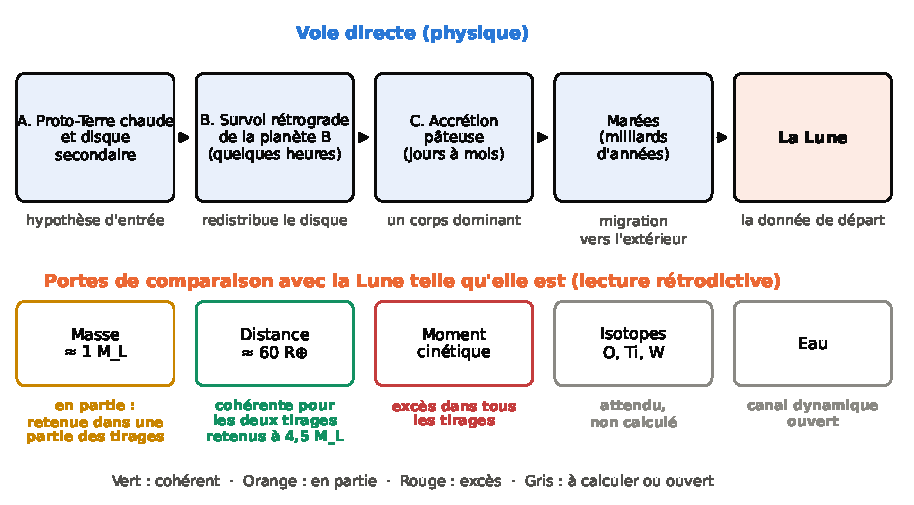
\includegraphics[width=\linewidth]{fig_chaine.pdf}
\caption{La logique de la théorie. En haut, le chemin direct~: proto-Terre et disque secondaire (phase~A, point de départ posé), survol rétrograde de la planète~$B$ (phase~B), assemblage du satellite en pâte (phase~C), marées. En bas, les portes de comparaison avec la Lune telle qu'elle est.\label{fig:chaine}}
\end{figure}

\subsection{Ce que veut dire « possible »}

Dire qu'un chemin est possible, c'est établir que, sous des conditions explicites, les lois de la physique le laissent ouvert et que son résultat tombe dans les ordres de grandeur de la donnée. Ce n'est pas dire que la Lune s'est formée ainsi. Les résultats de ce document sont donc de deux sortes. Ce sont des \emph{conditions nécessaires}~: par exemple, lue à rebours, la Lune exige que la Terre ait tourné avec un certain moment cinétique~; d'autres valeurs des paramètres libres peuvent mener au même état final, et le calcul ne dit pas laquelle a eu lieu. Ou bien ce sont des \emph{familles de solutions}, dont on dit les bords quand on les connaît. Le même critère vaut pour toute autre origine de la Lune.

Pour que le lecteur sache toujours sur quoi il se tient, chaque énoncé important porte l'un des trois statuts suivants~: \stCalc{} (résultat des calculs de ce document, dans le modèle décrit), \stSup{} (donnée d'entrée ou hypothèse, non démontrée ici), \stOuv{} (défini mais non calculé).

% =====================================================================
\section{Le décor physique}
\label{sec:decor}

Cette section décrit, en mots, les acteurs de la théorie et les hypothèses qui les définissent. Les calculs qui s'appuient sur eux viennent ensuite.

\subsection{Une proto-Terre chaude, molle, aplatie}
\label{sec:chaude}

Une planète qui grandit par accrétion convertit en chaleur l'énergie de la matière qui tombe sur elle. Pour une masse et un rayon terrestres, cela représente environ $3{,}7\times10^7$~J par kilogramme, soit près de cent fois ce qu'il faut pour fondre un silicate. L'énergie d'accrétion suffit donc, en ordre de grandeur, à fondre toute la planète et à en vaporiser une partie, \emph{si elle est suffisamment retenue}. Les modèles d'océan de magma montrent qu'une enveloppe de vapeur peut ralentir fortement le refroidissement \citep{ElkinsTanton2012,Hamano2013,Lebrun2013,Rubie2015}. La proto-Terre est donc chaude, et la théorie la suppose telle (hypothèse H1).

\textbf{Un corps mou, jamais liquide.} La proto-Terre de cette théorie est un corps \emph{mou}~: une matière pâteuse, comme une pâte à modeler épaisse, et non un liquide. Cette précision compte pour la suite. Un liquide suit une marée sans frotter~; un solide froid se déforme à peine~; une matière molle se déforme sous la marée et frotte, de sorte que son comportement n'est celui ni de l'un ni de l'autre. La marée soulevée dans un corps mou n'est pas celle d'un corps solide, ce qui a deux conséquences sur lesquelles nous reviendrons~: la marée est faible au début de l'histoire, et la dissipation dépend de la viscosité de la matière. Le passage de la planète~$B$ ne change en rien ce caractère mou~; il dure quelques heures et la Terre ne se refroidit pas pendant ce temps.

\textbf{Aplatie et gonflée.} Un corps mou qui tourne s'aplatit aux pôles et se gonfle à l'équateur. Avec une rotation de $6$~h, nous adoptons un rayon équatorial $\Req=1{,}60\,\Rt$ (et $1{,}52\,\Rt$ pour une rotation de $5$~h). Ces rayons sont des \emph{hypothèses d'entrée}, non des structures calculées~; la section~\ref{sec:poids} montre pourquoi la théorie les exige. La rotation de $5$ à $6$~h est elle aussi posée (H2)~: l'accrétion peut la fournir, sans impact. Une objection existe~: \citet{DonesTremaine1993} ont montré que l'accrétion régulière de petits corps ne donne pas à une planète comme la Terre sa vitesse de rotation actuelle. H2 reste donc une hypothèse. La rétrodiction de la section~\ref{sec:AM} part de la Lune et ne l'utilise pas, mais l'excès de moment cinétique qu'elle chiffre en dépend.

\begin{table}[htbp]
\centering
\caption{Figure de la proto-Terre pour les deux cas de référence (calculée à partir de H1 et H2). Le nombre de rotation compare la vitesse de rotation à celle à laquelle une particule équatoriale orbiterait~; il vaudrait~1 à la rupture.\label{tab:forme}}
\small
\begin{tabular}{lcc}
\toprule
Grandeur & 5 h, $1{,}52\,\Rt$ & 6 h, $1{,}60\,\Rt$ \\
\midrule
Nombre de rotation & $0{,}53$ & $0{,}47$ \\
Aplatissement (rayon polaire / équatorial) & $0{,}88$ & $0{,}90$ \\
Gravité équatoriale restante & $72\,\%$ & $78\,\%$ \\
Densité moyenne & $1{,}8$--$1{,}9$~g\,cm$^{-3}$ & $1{,}5$~g\,cm$^{-3}$ \\
Rayon de corotation & $2{,}33\,\Rt$ & $2{,}63\,\Rt$ \\
\bottomrule
\end{tabular}
\end{table}

Le \emph{rayon de corotation} du tableau~\ref{tab:forme} est la distance à laquelle un corps en orbite tourne exactement aussi vite que la Terre. Il joue un rôle central plus loin~: un satellite qui se fixe au-delà de ce rayon est repoussé par la marée, un satellite qui se fixe en deçà est attiré vers la Terre.

\subsection{Le disque secondaire et la limite de Roche}
\label{sec:roche}

Autour de la proto-Terre se trouve un \emph{disque secondaire}~: un réservoir de matière né en même temps qu'elle, qui n'a pas encore formé de satellite. La théorie le place au-delà de la \emph{limite de Roche}. C'est la distance en deçà de laquelle la marée de la planète déchire un corps fluide plus vite que sa propre gravité ne peut le rassembler~; au-delà, les corps peuvent grandir \citep{SalmonCanup2012}. Pour une matière de densité lunaire ($3{,}34$~g\,cm$^{-3}$), cette limite est à $2{,}90\,\Rt$. Elle ne dépend que de la masse de la Terre et de la densité du satellite, \emph{pas} du gonflement de la proto-Terre. Une matière plus légère a une limite plus lointaine~: $3{,}15\,\Rt$ à $2{,}6$~g\,cm$^{-3}$, $3{,}79\,\Rt$ à $1{,}5$~g\,cm$^{-3}$.

Le disque s'étend de la limite de Roche jusqu'à environ $5\,\Rt$. Sa densité de surface augmente vers l'extérieur, comme on l'attend quand le transport de moment cinétique étale la matière vers de grands rayons. Il est épais en latitude, dans la bande intertropicale ($\pm26^\circ$), parce que le passage de la planète~$B$ est incliné de $25^\circ$ et que c'est là que sa marée se fait sentir. Sa formation (phase~A) n'est pas calculée~: sa masse totale, de $4$ à $5{,}4$ masses lunaires, est un paramètre (H3). La figure~\ref{fig:zones} donne la carte des distances.

\begin{figure}[htbp]
\centering
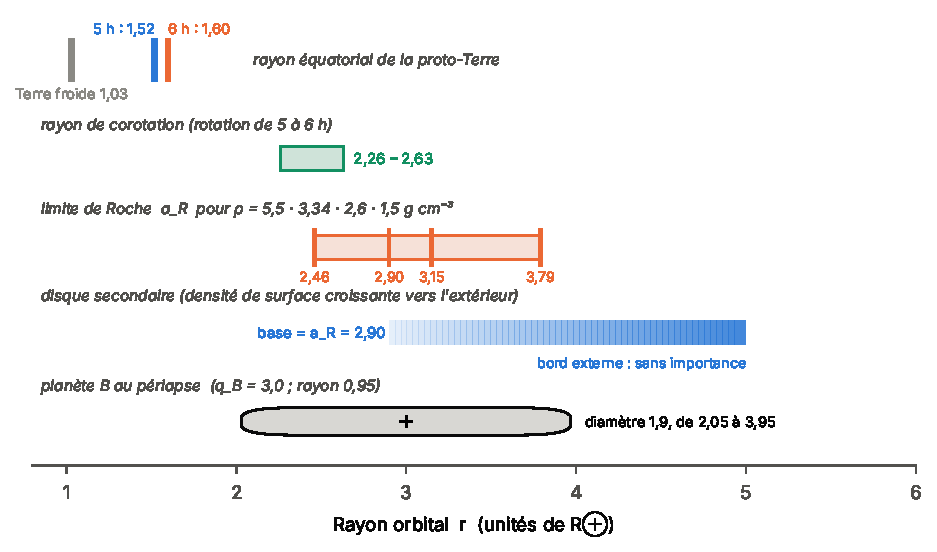
\includegraphics[width=\linewidth]{fig_zones.pdf}
\caption{Carte radiale du système, en rayons terrestres~: rayons équatoriaux de la proto-Terre (5~h, 6~h), rayon de corotation, étendue de la limite de Roche selon la densité de la matière, disque secondaire (densité de surface croissante vers l'extérieur) et planète~$B$ à son point le plus proche.\label{fig:zones}}
\end{figure}

\textbf{Un disque d'abord non collant, ensuite pâteux (proposition P2).} Jusqu'au passage de la planète~$B$, le disque est baigné par le gaz du jeune Soleil, par la vapeur de l'océan de magma et par le rayonnement de la proto-Terre, dont la surface est à $2000$--$3000$~K. Dans ces conditions les corps qui se touchent rebondissent ou s'érodent au lieu de fusionner~: le disque reste dispersé. Le passage a lieu pendant la phase de gaz, dans les premiers millions d'années du Système solaire \citep{Weiss2021,Mamajek2009}. Après le passage, la matière redistribuée est traitée comme une \emph{pâte molle}~: deux morceaux qui se touchent collent (H4). Un corollaire sur l'âge~: la Lune se forme peu après la Terre, et les âges de $4{,}51$ et $4{,}46$ milliards d'années \citep{Barboni2017,Greer2023} datent la différenciation et la cristallisation de l'océan magmatique lunaire, non l'accrétion.

\textbf{Un disque pauvre en fer métallique (proposition P1).} La Lune a peu de fer métallique, et sa densité est de $3{,}34$~g\,cm$^{-3}$. La théorie suppose que le disque a été appauvri en métal avant le passage~: le métal, plus dense, a rejoint le noyau de la proto-Terre. Cette proposition n'est pas calculée~; elle a une conséquence testable sur les éléments qui suivent le fer (Ni, Co, W).

\subsection{La planète~$B$ et ce qu'elle fait}
\label{sec:B}

La planète~$B$ est une planète rocheuse de $0{,}95$ masse terrestre, recouverte d'une mince pellicule de glace (H5). Elle est un peu plus dense que la Terre ($6{,}1$~g\,cm$^{-3}$) plutôt que plus grande, ce qui lui permet de passer près de la Terre sans se briser~: à $3{,}0\,\Rt$ du centre, elle garde une marge de $18\,\%$ sur la distance de contact avec une proto-Terre de $1{,}60\,\Rt$. Elle suit une trajectoire ouverte (une hyperbole), à la vitesse de $2$~km\,s$^{-1}$ loin de la Terre et de $9{,}2$~km\,s$^{-1}$ à son point le plus proche. Elle est de sens \emph{rétrograde}, c'est-à-dire à contresens de la rotation de la Terre, et inclinée de $25^\circ$ sur l'équateur (H6).

\textbf{Aucune matière n'est transférée (H7).} La planète~$B$ ne fournit aucune matière à la proto-Terre ni au satellite en formation. Elle n'agit que par gravitation. La seule chose qu'elle laisse est la vapeur d'eau de sa pellicule de glace, qui arrive surtout sur la Terre (H8, section~\ref{sec:eau}). Cette règle est le cœur du caractère isotopique de la théorie (section~\ref{sec:isotopes}).

\textbf{Trois effets, tous gravitationnels.} Pendant les quelques heures du survol, la planète~$B$ agit de trois façons.
\begin{enumerate}[leftmargin=1.6em,itemsep=2pt]
\item Elle \emph{redistribue la matière du disque}~: une partie tombe sur la Terre, une partie reste liée sur des orbites nouvelles et plus inclinées, une partie s'échappe.
\item Elle \emph{fait basculer l'axe de rotation} de la Terre, par son attraction sur le renflement équatorial.
\item Elle \emph{emporte un peu du moment cinétique} de la rotation de la Terre~: la marée qu'elle soulève freine la rotation, et le moment cinétique ainsi retiré à la Terre passe dans le mouvement de la planète~$B$.
\end{enumerate}
Les phases suivantes (assemblage du satellite, marées) conservent ou transfèrent ce qui reste~; elles n'en retirent presque rien. Nous verrons que la quantité retirée par le troisième effet dépend de la nature de la matière de la proto-Terre, et qu'elle est modeste.

\textbf{Pourquoi rétrograde.} La planète~$B$ se déplace, à son point le plus proche, à une vitesse angulaire de $4{,}8\times10^{-4}$~s$^{-1}$, tandis que la matière du disque tourne à $2{,}4\times10^{-4}$~s$^{-1}$ à $3\,\Rt$ et à $1{,}1\times10^{-4}$~s$^{-1}$ à $5\,\Rt$. Dans le sens de la rotation (prograde), la planète~$B$ rattrape lentement la matière, et les mêmes parcelles sont tirées de façon cohérente pendant longtemps~: elles sont arrachées. À contresens (rétrograde), la planète~$B$ rencontre la matière de face~: chaque parcelle reçoit un coup bref, et les coups s'accumulent moins. Le passage rétrograde \emph{réarrange} donc les orbites sans emporter le disque. Le contraste numérique est donné à la section~\ref{sec:phaseB}.

\textbf{Géométrie.} L'argument du périapse $\omega_B=90^\circ$ place le point le plus proche de la Terre au sommet de l'orbite, à la latitude $+25^\circ$ au-dessus de l'équateur (figure~\ref{fig:geometry}). La planète~$B$ passe donc \emph{au-dessus} du disque, à environ $3\,\Rt$ de la Terre, et son centre ne traverse le plan du disque qu'après l'avoir quitté, à environ $6\,\Rt$ de la Terre (le disque s'arrête à $5\,\Rt$). Une orbite à $\omega_B=0$ passerait au contraire dans le plan du disque~; ce n'est pas l'hypothèse de la théorie.

\begin{table}[htbp]
\centering
\caption{La planète~$B$ et la géométrie du passage de référence (calculé, orbite hyperbolique non perturbée).\label{tab:B}}
\small
\begin{tabular}{lc}
\toprule
Grandeur & Valeur \\
\midrule
Masse, rayon, densité & $0{,}95\,\Mt$, $0{,}95\,\Rt$, $6{,}1$~g\,cm$^{-3}$ \\
Gravité de surface & $1{,}05\,g_\oplus$ \\
Distance du point le plus proche $\qB$ & $3{,}0\,\Rt$ \\
Vitesse à l'infini, vitesse au point le plus proche & $2$ et $9{,}24$~km\,s$^{-1}$ \\
Excentricité de l'hyperbole & $1{,}098$ \\
Inclinaison sur l'équateur (rétrograde), argument du périapse & $25^\circ$, $90^\circ$ \\
Hauteur du centre de la planète~$B$ au-dessus de l'équateur au périapse & $1{,}27\,\Rt$ \\
Distance à laquelle son centre traverse le plan de l'équateur & $6{,}3\,\Rt$ \\
\bottomrule
\end{tabular}
\end{table}

\begin{figure}[htbp]
\centering
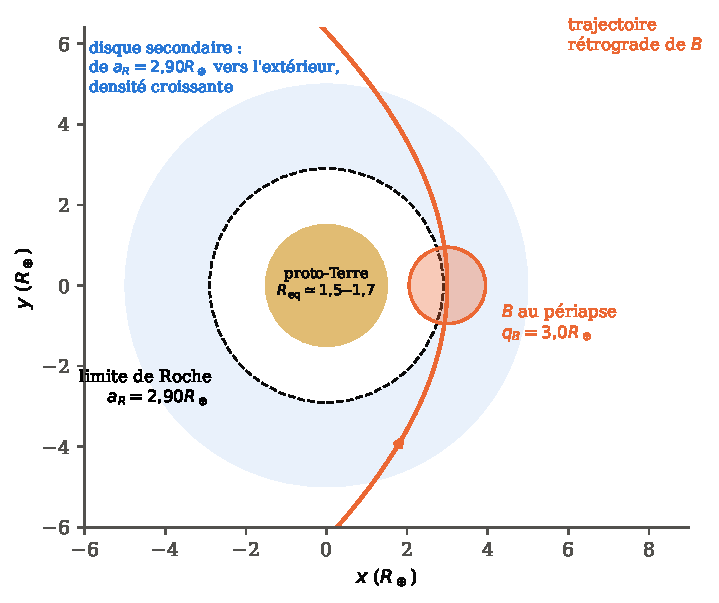
\includegraphics[width=0.78\linewidth]{fig_geometry.pdf}
\caption{Géométrie du passage dans le plan équatorial de la Terre (à l'échelle~; la trajectoire réelle est inclinée de $25^\circ$). Le disque secondaire commence à la limite de Roche ($2{,}90\,\Rt$, tirets). La planète~$B$ atteint son point le plus proche à $3{,}0\,\Rt$, à la base du disque, en se déplaçant à contresens de la rotation de la Terre.\label{fig:geometry}}
\end{figure}

\subsection{Les hypothèses en un tableau}

Le tableau~\ref{tab:hypotheses} liste les conditions posées. Aucune n'est cachée dans le code~: chacune est une donnée d'entrée ou une règle de calcul, et son statut est dit.

\begin{table}[htbp]
\centering
\caption{Les hypothèses (H) et propositions (P) d'entrée.\label{tab:hypotheses}}
\small
\begin{tabular}{>{\raggedright\arraybackslash}p{0.9cm}>{\raggedright\arraybackslash}p{10.6cm}>{\raggedright\arraybackslash}p{2.9cm}}
\toprule
N$^\circ$ & Énoncé & Statut \\
\midrule
H1 & Proto-Terre chauffée par son accrétion, corps mou et non liquide, aplatie et gonflée à $\Req=1{,}52\,\Rt$ (5~h) ou $1{,}60\,\Rt$ (6~h) & \stSup \\
H2 & Rotation initiale de $5$--$6$~h, fournie par l'accrétion et non par un impact & \stSup \\
H3 & Disque secondaire préexistant, de base à la limite de Roche, dans la bande $\pm26^\circ$. Sa masse est un paramètre~: de $4{,}5$ à $5{,}4$ masses lunaires ont donné un satellite conservé & \stSup, masse partiellement \stCalc \\
H4 & Après le survol, la matière est une pâte molle~: deux morceaux qui se touchent collent & \stSup \\
H5 & La planète~$B$~: $0{,}95\,\Mt$, $0{,}95\,\Rt$, $6{,}1$~g\,cm$^{-3}$, mince pellicule de glace & \stSup \\
H6 & Survol rétrograde, sans contact~: distance $3{,}0\,\Rt$, vitesse $2$~km\,s$^{-1}$ à l'infini, inclinaison $25^\circ$, $\omega_B=90^\circ$ & \stSup \\
H7 & Aucun transfert de matière depuis la planète~$B$~; elle n'agit que par gravitation & \stSup \\
H8 & L'eau de la pellicule de glace arrive surtout sur la Terre & \stSup, canal \stOuv \\
P1 & Le disque est appauvri en fer métallique avant le survol & \stSup, mécanisme \stOuv \\
P2 & Jusqu'au survol, le disque est non collant (gaz, vapeur, rayonnement)~; le survol a lieu pendant la phase de gaz & \stSup, mécanisme \stOuv \\
\bottomrule
\end{tabular}
\end{table}

% =====================================================================
\section{La méthode en bref}
\label{sec:methode}

Le calcul suit trois phases, que la figure~\ref{fig:chaine} place sur une même ligne. La \emph{phase~A} est l'existence de la proto-Terre et de son disque~; elle est posée, non calculée. La \emph{phase~B} est le survol, qui dure quelques heures. La \emph{phase~C} est ce qui suit, de quelques jours à des milliards d'années.

\textbf{Phase~B~: des particules-test.} Le disque est représenté par $700$ traceurs de masses égales, répartis dans la bande intertropicale entre la limite de Roche et $5\,\Rt$. On les suit pendant que la planète~$B$ parcourt son hyperbole, de huit distances de périapse avant le passage à huit après. Les traceurs ne se heurtent pas pendant les quelques heures du survol, ce que justifie l'état non collant du disque avant le passage (P2). Après le survol, chaque traceur est classé selon son énergie~: lié à la Terre, échappé, ou tombé sur la surface. La planète~$B$ est traitée comme une masse qui attire, rien de plus.

\textbf{Phase~C~: un calcul à $N$ corps.} Les traceurs liés deviennent $700$ petits corps, suivis par un code de dynamique à $N$ corps. Les corps qui se touchent fusionnent comme une pâte molle (H4). La marée de la Terre est incluse. On suit le résultat pendant un an, puis, pour les réalisations qui gardent un satellite, pendant cinq ans.

\textbf{Marées séculaires.} À partir de l'état obtenu à cinq ans, un modèle qui moyenne les mouvements rapides fait évoluer l'orbite du satellite et la rotation de la Terre sous l'effet des marées de la Lune et du Soleil, pendant $4{,}5$ milliards d'années. Les paramètres de marée sont calibrés sur la dissipation de la Terre actuelle~; la distance atteinte varie lentement avec eux (un facteur $2$ sur la dissipation change la distance de $11\,\%$).

\textbf{Pourquoi ces outils.} Chaque outil est choisi pour ce que la phase demande. Pendant les quelques heures du survol, les traceurs ne s'influencent pas~: ils n'ont pas le temps de se rencontrer, et la seule force qui compte est l'attraction de la Terre et de la planète~$B$. Un calcul de particules-test est alors exact et rapide, ce qui permet de balayer beaucoup de géométries. Après le survol, au contraire, les corps se rencontrent, fusionnent et s'attirent mutuellement~: un calcul à $N$ corps est indispensable, et il est plus long. Enfin, sur des milliards d'années, il serait impossible de suivre chaque révolution~; un modèle qui moyenne les mouvements rapides suffit pour l'évolution lente des orbites.

\textbf{Qu'appelle-t-on une réalisation\,?} La distribution initiale des $700$ traceurs est tirée au hasard, et chaque tirage porte un numéro, la \emph{graine}. Deux graines donnent des disques statistiquement identiques mais des assemblages différents, parce que la phase~C est chaotique~: une petite différence initiale peut changer le corps qui finit par dominer. Chaque calcul complet est une \emph{réalisation}. C'est pourquoi les résultats de la phase~C sont donnés avec leur dispersion et sur plusieurs réalisations, jamais sur une seule.

\textbf{Comment les calculs sont vérifiés.} Les fractions de la phase~B varient de moins de $0{,}015$ quand on change la résolution, le pas de temps (de $20$ à $5$~s) ou la distance d'arrêt (de $30$ à $100\,\Rt$). Le moment cinétique de la phase~C est conservé à $10^{-4}\,\LEM$ près sur quatre ans, celui du bilan couplé à $10^{-6}\,\LEM$ près. Le calcul de dissipation de la matière molle reproduit à quatre chiffres le freinage du modèle à retard constant quand on lui donne le même noyau, et retrouve la solution exacte d'un corps uniforme. La marée solaire seule redonne, dans le bilan couplé, les valeurs de la section~\ref{sec:puits}.

\textbf{Calculs spécialisés.} Quatre calculs à part complètent la chaîne~: le poids du magma sous la planète~$B$~; le freinage de la rotation et la bascule de l'axe, avec un modèle de corps mou (rhéologie de Maxwell)~; la tenue d'un tas de gravats près de la limite de Roche~; et, nouveauté de cette version, un \emph{bilan couplé} du moment cinétique sur une seule trajectoire (section~\ref{sec:couple}).

\begin{table}[htbp]
\centering
\caption{Configuration de référence. Ces valeurs sont fixées dans tous les calculs, sauf mention d'un balayage.\label{tab:config}}
\small
\begin{tabular}{>{\raggedright\arraybackslash}p{4.4cm}>{\raggedright\arraybackslash}p{5.6cm}>{\raggedright\arraybackslash}p{4.6cm}}
\toprule
Grandeur & Valeur & Commentaire \\
\midrule
Rotation et rayon équatorial & $6$~h, $1{,}60\,\Rt$ (ou $5$~h, $1{,}52\,\Rt$) & hypothèses \\
Planète~$B$ & $0{,}95\,\Mt$, $0{,}95\,\Rt$, $6{,}1$~g\,cm$^{-3}$ & pellicule de glace négligée en masse \\
Survol & distance $3{,}0\,\Rt$, $2$~km\,s$^{-1}$, $25^\circ$ rétrograde, $\omega_B=90^\circ$ & point le plus proche à $+25^\circ$ \\
Disque & de $2{,}90\,\Rt$ à $5\,\Rt$, densité de surface croissante, $|\lambda|\le26^\circ$ & masse de $4{,}0$ à $5{,}4$ masses lunaires \\
Matière du disque & pâte molle à $3\,340$~kg\,m$^{-3}$ & densité lunaire \\
Marée de la Terre & $k_2=0{,}032$, retard $959$~s (soit $k_2/Q\simeq10^{-2}$) & calibration indépendante \\
\bottomrule
\end{tabular}
\end{table}

% =====================================================================
\section{Le survol et la naissance du satellite}
\label{sec:survol}

Cette section suit la chaîne dans l'ordre du temps~: l'effet du survol sur la surface de la Terre, la redistribution du disque, l'assemblage du corps, sa conservation, puis sa migration jusqu'à la distance lunaire. Chaque résultat est suivi de ce qu'il faut en retenir.

\subsection{La marée de la planète~$B$ allège le magma situé sous elle}
\label{sec:poids}

Au point de la surface qui se trouve juste sous la planète~$B$, trois accélérations se combinent~: la gravité de la Terre, qui retient la matière~; la poussée centrifuge de la rotation, qui l'allège à l'équateur~; et l'attraction de la planète~$B$, qui la tire vers le haut. Quand la traction l'emporte, la matière n'est plus retenue au sol. À une distance donnée de la planète~$B$, on peut définir un \emph{rayon de poids nul}~: tout point de la surface situé plus loin que lui du centre est délesté.

À $3{,}0\,\Rt$, le rayon de poids nul est de $1{,}51\,\Rt$ pour une rotation de $5$~h et de $1{,}54\,\Rt$ pour $6$~h (figure~\ref{fig:weight}). La surface n'est donc délestée au point le plus proche que si le rayon équatorial de la proto-Terre dépasse ces valeurs. Les deux cas de référence y satisfont~: à $6$~h et $1{,}60\,\Rt$, la surface est délestée sur toute la bande intertropicale, avec une marge de $0{,}01$ à $0{,}06\,\Rt$. L'attraction de la planète~$B$ y vaut alors $0{,}97$ fois la gravité de surface.

\begin{figure}[htbp]
\centering
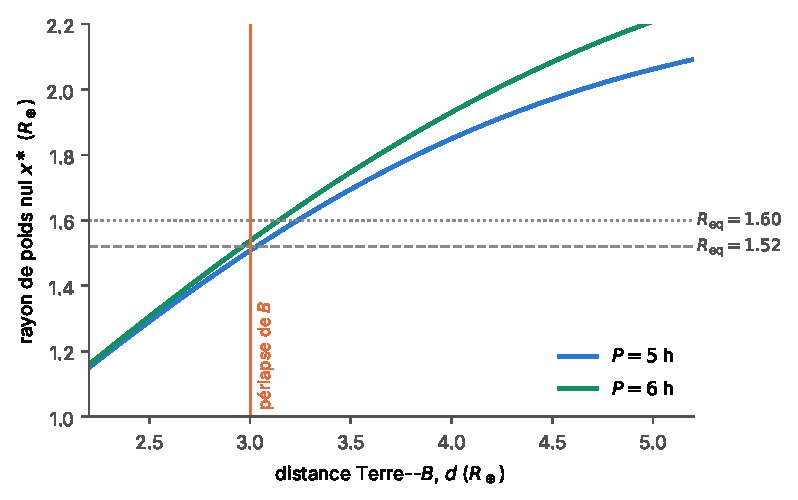
\includegraphics[width=0.85\linewidth]{fig_weight.pdf}
\caption{Rayon de poids nul sous la planète~$B$ en fonction de sa distance, pour les rotations de $5$~h et $6$~h. Un point de la surface est délesté lorsque la courbe passe sous le rayon équatorial de la proto-Terre. À $3{,}0\,\Rt$, les courbes sont à $1{,}51\,\Rt$ ($5$~h) et $1{,}54\,\Rt$ ($6$~h).\label{fig:weight}}
\end{figure}

\textbf{À retenir.} Cette condition est précise et réfutable~: une proto-Terre froide et compacte ($\Req\simeq1{,}03\,\Rt$) ne serait pas délestée à cette distance, et la théorie exige donc une Terre gonflée par sa chaleur. Le calcul est quasi statique~; il fixe le rayon requis, mais ne dit pas quelle quantité de magma est soulevée ni ce qu'elle devient. Les calculs qui suivent n'en dépendent pas.

\subsection{Phase~B~: un passage rétrograde redistribue le disque}
\label{sec:phaseB}

Après le passage d'une heure, sur $100$ parts du disque, environ $47$ sont encore sur des orbites autour de la Terre, sur des orbites inclinées d'environ $31^\circ$~; environ $21$ ont été envoyées vers la surface de l'océan de magma~; environ $33$ ont quitté la Terre. Un passage de même géométrie mais dans le sens de la rotation n'en garderait que $14$ (tableau~\ref{tab:phaseB}, figure~\ref{fig:phaseB}). Le passage rétrograde garde donc environ $3{,}5$ fois plus de matière autour de la Terre.

\begin{table}[htbp]
\centering
\caption{Devenir des traceurs du disque après le passage (distance $3{,}0\,\Rt$, $0{,}95\,\Mt$, disque de $2{,}90$ à $5\,\Rt$, moyennes sur trois graines de $700$ traceurs, dispersion de $0{,}01$--$0{,}02$). « Tombés »~: tombés sur la Terre~; « liés »~: liés à la Terre~; « perdus »~: ayant quitté la Terre~; « périapse $>a_R$ »~: fraction du disque entier qui est liée et qui reste en dehors de la zone où un corps fluide serait déchiré.\label{tab:phaseB}}
\small
\begin{tabular}{lccccc}
\toprule
Passage & tombés & liés & perdus & périapse $>a_R$ & inclin. \\
\midrule
Rétrograde $25^\circ$ & 0,21 & \textbf{0,47} & 0,33 & 0,15 & $31{,}5^\circ$ \\
Rétrograde coplanaire & 0,15 & 0,44 & 0,42 & 0,14 & $20{,}0^\circ$ \\
Prograde $25^\circ$ & 0,18 & 0,14 & 0,68 & 0,10 & $20{,}5^\circ$ \\
\bottomrule
\end{tabular}
\end{table}

\begin{figure}[htbp]
\centering
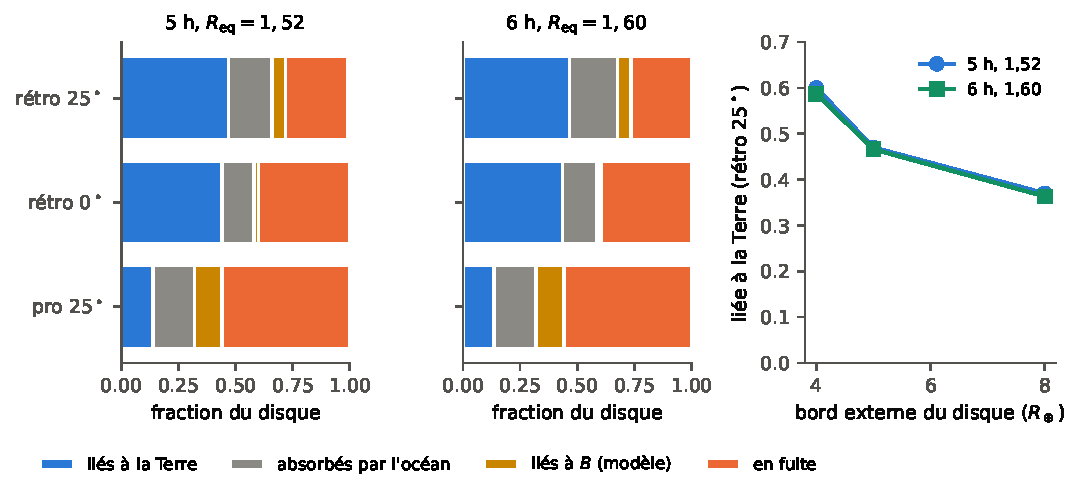
\includegraphics[width=\linewidth]{fig_phaseB.pdf}
\caption{Phase~B. À gauche et au milieu~: devenir des traceurs pour les deux cas de référence et trois passages (rétrograde à $25^\circ$, rétrograde coplanaire, prograde à $25^\circ$). À droite~: fraction du disque liée à la Terre pour le passage rétrograde en fonction du bord externe du disque.\label{fig:phaseB}}
\end{figure}

Le résultat est insensible à la pente de la densité de surface (la fraction liée vaut $0{,}46$ à $0{,}48$ pour les trois pentes essayées). Il dépend en revanche du bord externe du disque~: $0{,}60$, $0{,}47$ et $0{,}37$ pour $4$, $5$ et $8\,\Rt$, parce que la matière située plus loin que le point le plus proche de la planète~$B$ est plus facilement emportée.

Un second tri éclaire la dynamique. On place $504$ particules sur des orbites circulaires entre la surface de la Terre gonflée et la limite de Roche, et l'on regarde où elles vont (tableau~\ref{tab:504}). Le passage rétrograde à $25^\circ$ est le plus efficace~: il place $18{,}5\,\%$ du réservoir dans la « fenêtre lunaire » (matière liée, hors de la Terre, avec un rayon circulaire au-delà de la limite de Roche), garde $80\,\%$ autour de la Terre et n'en laisse rien échapper. Le passage prograde disperse le réservoir~: $4\,\%$ seulement dans la fenêtre, plus de la moitié perdue. L'efficacité est maximale à $25^\circ$ et ne forme pas un plateau, ce qui ancre le choix de cette inclinaison.

\begin{table}[htbp]
\centering
\caption{Partition de $504$ particules placées entre la surface et la limite de Roche, après le survol (moyenne de cinq grilles).\label{tab:504}}
\small
\begin{tabular}{lcccc}
\toprule
Passage & fenêtre lunaire & disque intérieur lié & tombées sur la Terre & perdues \\
\midrule
Rétrograde $20^\circ$ & 0,130 & 0,516 & 0,279 & 0,075 \\
Rétrograde $25^\circ$ & \textbf{0,185} & 0,612 & 0,204 & 0,000 \\
Rétrograde $30^\circ$ & 0,133 & 0,605 & 0,262 & 0,000 \\
Prograde $25^\circ$ & 0,042 & 0,014 & 0,397 & 0,547 \\
\bottomrule
\end{tabular}
\end{table}

Le survol \emph{agite} le disque. On mesure l'agitation par un indice qui combine l'excentricité et l'inclinaison des orbites~: il passe de $0{,}23$ avant le survol à $0{,}72$ après, et les orbites liées ont alors une excentricité médiane de $0{,}40$. Les morceaux voisins se croisent donc à des vitesses de l'ordre de $0{,}7$ fois la vitesse képlérienne. C'est pourquoi la règle de pâte (H4), qui fait coller les corps au contact, est essentielle à l'assemblage qui suit.

\textbf{À retenir.} Le survol rétrograde garde autour de la Terre environ la moitié du disque, sur des orbites inclinées, contre un septième pour le passage prograde. Une moitié de disque liée à la Terre est la matière première de la Lune~; le tiers de cette moitié (environ $0{,}15$ du disque) est sur des orbites dont le point le plus bas reste au-delà de la limite de Roche, donc assemblable tout de suite.

\subsection{Phase~C~: la pâte s'assemble en un corps dominant}
\label{sec:phaseC}

Dans les premières semaines, la matière redistribuée, qui colle au contact, se rassemble en un seul corps. Le corps se stabilise ensuite près de la limite de Roche sur une orbite presque circulaire, et son plan orbital se rapproche lentement de l'équateur (tableau~\ref{tab:phaseC}, figures~\ref{fig:sequence} et~\ref{fig:phaseC}).

\begin{figure}[htbp]
\centering
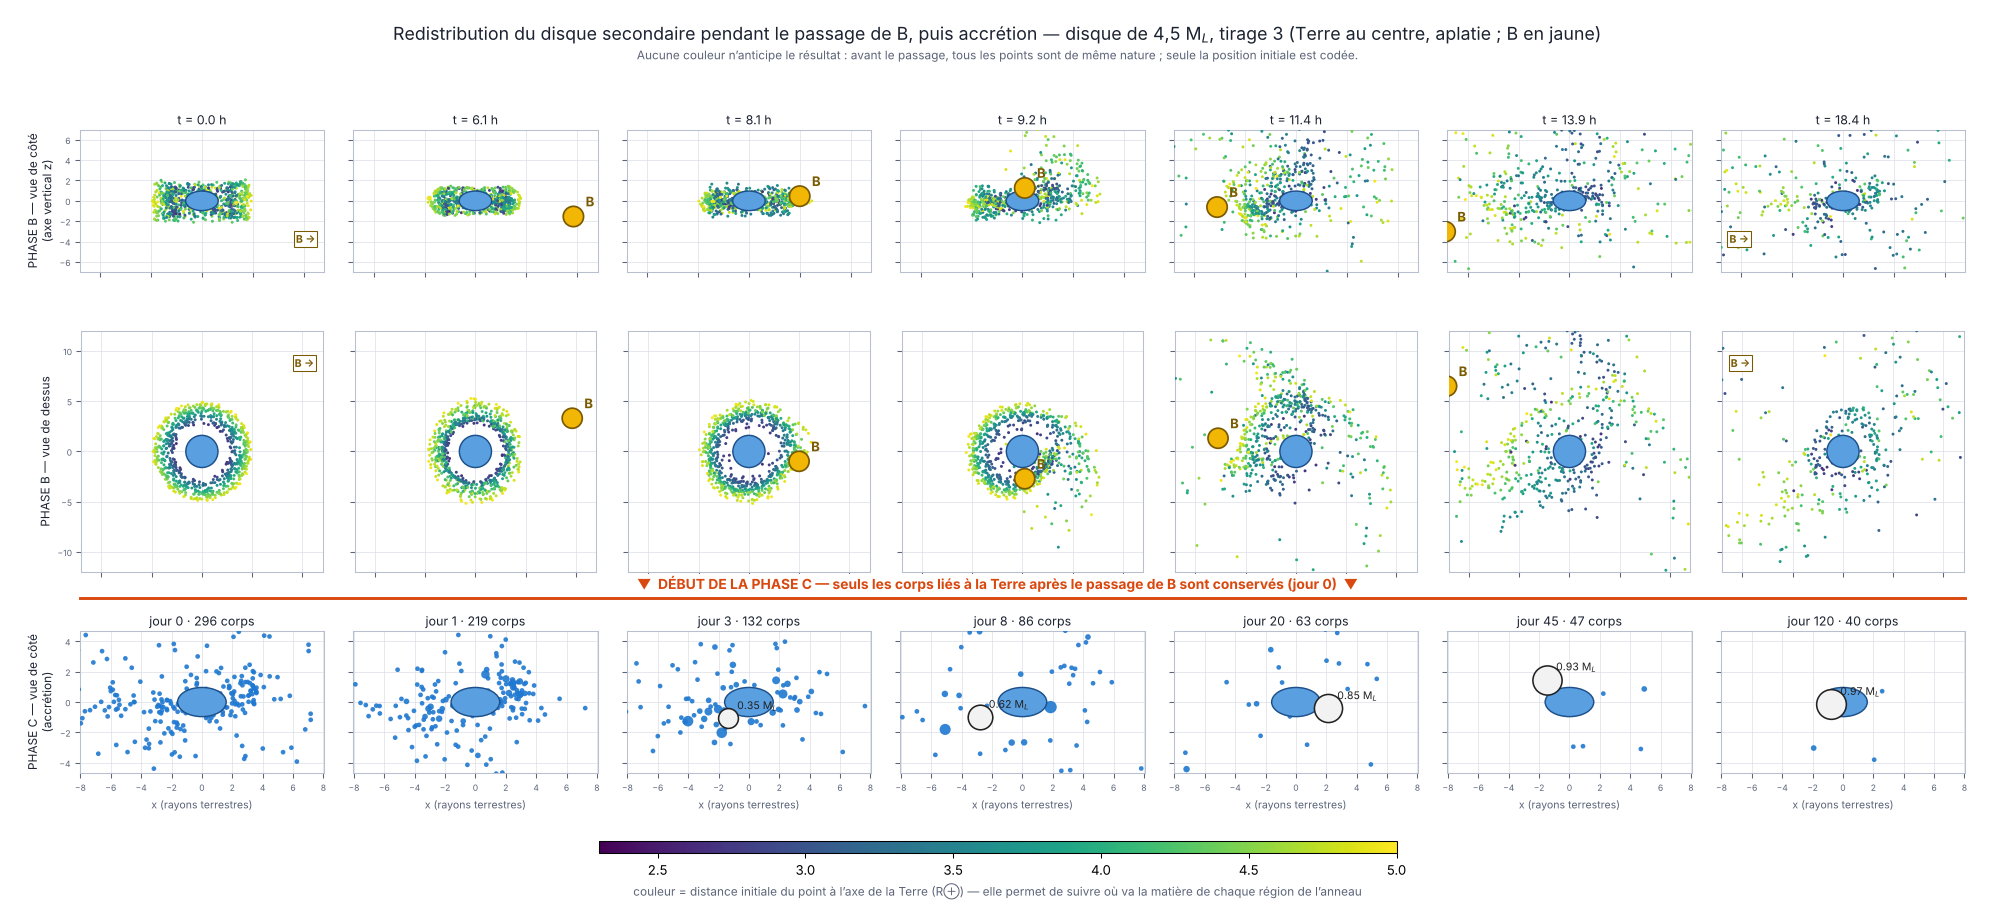
\includegraphics[width=\linewidth]{fig_sequence.png}
\caption{Séquence de la phase~C pour la réalisation de référence~: la matière liée après le survol s'assemble en un corps dominant en quelques semaines.\label{fig:sequence}}
\end{figure}

\begin{table}[htbp]
\centering
\caption{Corps dominant au cours de la première année (réalisation de référence, graine~0). $M_1$~: masse du corps dominant~; $a_1$, $e_1$, $i_1$~: son demi-grand axe, son excentricité et son inclinaison sur l'équateur.\label{tab:phaseC}}
\small
\begin{tabular}{lcccccc}
\toprule
Cas & jour & $M_1$ ($\ML$) & $a_1$ ($\Rt$) & $e_1$ & $i_1$ ($^\circ$) \\
\midrule
5 h, $1{,}52\,\Rt$ & 10 & 0,93 & 2,97 & 0,10 & 27,7 \\
 & 90 & 1,20 & 2,77 & 0,10 & 28,1 \\
 & 365 & 1,30 & 3,10 & 0,11 & 12,8 \\
\addlinespace
6 h, $1{,}60\,\Rt$ & 10 & 1,30 & 3,01 & 0,02 & 26,6 \\
 & 90 & 1,40 & 2,99 & 0,05 & 22,0 \\
 & 365 & 1,43 & 3,17 & 0,08 & 10,4 \\
\bottomrule
\end{tabular}
\end{table}

\begin{figure}[htbp]
\centering
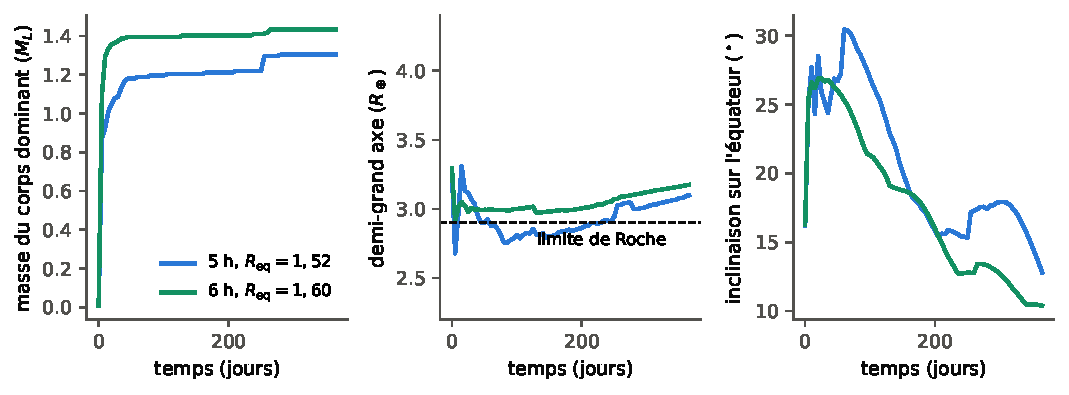
\includegraphics[width=\linewidth]{fig_phaseC.pdf}
\caption{Phase~C avec marées (un an) pour les deux cas de référence. À gauche~: masse du corps dominant. Au milieu~: son demi-grand axe, comparé à la limite de Roche. À droite~: son inclinaison sur l'équateur.\label{fig:phaseC}}
\end{figure}

\textbf{Dispersion, masse du disque, règle de surface.} Trois réalisations supplémentaires par cas donnent, après un an, un corps de $1{,}36$ à $1{,}69$ masse lunaire à $5$~h et de $1{,}23$ à $1{,}38$ à $6$~h~: un corps de masse lunaire se forme dans les huit réalisations, sur une orbite presque circulaire dont l'inclinaison retombe à $3$--$13^\circ$. Faire varier la masse du disque à $5$~h donne $0{,}03$, $1{,}52$ et $1{,}28$ masse lunaire pour $2{,}7$, $5{,}4$ et $8{,}1$ masses lunaires de disque~: avec un disque trop léger, la matière retenue est trop peu dense pour s'assembler, et le résultat de masse lunaire tient de $5$ à $8$ masses lunaires à $5$~h. Enfin, dans le calcul de référence, les corps qui touchent la surface de la Terre sont réaccrétés par elle (H7 le permet)~; avec la règle opposée, qui les supprime, le cas à $5$~h donne $1{,}60$ masse lunaire, c'est-à-dire le même résultat.

\textbf{À retenir.} Un corps de $1{,}30$ à $1{,}43$ masse lunaire domine dès les premières semaines, avec des compagnons de $0{,}14$ et $0{,}02$ masse lunaire. L'orbite est stable sur l'année, à $3$ rayons terrestres environ, et l'inclinaison décroît sous l'effet de la marée de $27^\circ$ à $10^\circ$. Le corps n'est pas encore sur l'équateur~; les marées doivent l'y amener.

\subsection{Ce que change le passage~: le témoin sans la planète~$B$}
\label{sec:control}

Pour savoir ce que change le survol, on refait la phase~C sur le même disque sans la planète~$B$ (tableau~\ref{tab:control}, figure~\ref{fig:temoin}). Livré à lui-même, le disque de $5{,}4$ masses lunaires est dynamiquement froid et collant~: il s'effondre en quelques jours en un seul corps de $3{,}5$ à $3{,}9$ masses lunaires, sur une orbite presque circulaire et équatoriale, à $4{,}6$--$4{,}7\,\Rt$. Avec la planète~$B$, la même masse de départ donne un corps de $1{,}3$ à $1{,}4$ masse lunaire, et le système contient $1{,}35\,\LEM$ au lieu d'environ $2{,}0\,\LEM$.

\begin{table}[htbp]
\centering
\caption{Phase~C après un an, avec et sans le passage (même disque de $5{,}4$ masses lunaires, mêmes règles). $L$~: moment cinétique du corps dominant plus rotation de la Terre.\label{tab:control}}
\small
\begin{tabular}{lcccccc}
\toprule
Cas & $M_1$ ($\ML$) & $a_1$ ($\Rt$) & $e_1$ & $i_1$ ($^\circ$) & $L$ ($\LEM$) \\
\midrule
5 h, avec la planète~$B$ & 1,30 & 3,10 & 0,11 & 12,8 & 1,35 \\
5 h, sans la planète~$B$ & 3,47 & 4,58 & 0,10 & 0,7 & 2,04 \\
6 h, avec la planète~$B$ & 1,43 & 3,17 & 0,08 & 10,4 & 1,35 \\
6 h, sans la planète~$B$ & 3,86 & 4,68 & 0,13 & 0,4 & 1,97 \\
\bottomrule
\end{tabular}
\end{table}

\begin{figure}[htbp]
\centering
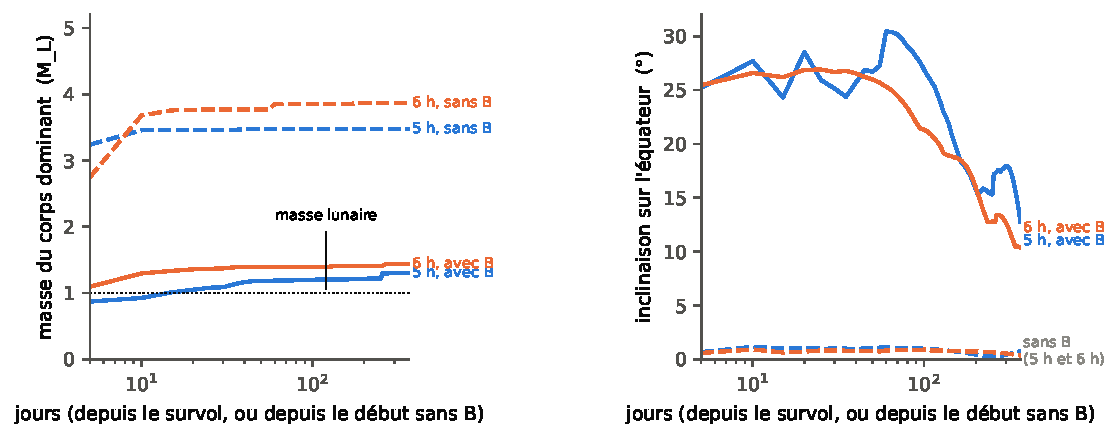
\includegraphics[width=\linewidth]{fig_temoin.pdf}
\caption{Phase~C avec et sans le passage (même disque, mêmes règles). Gauche~: masse du corps dominant, la ligne en pointillés marquant la masse lunaire. Droite~: son inclinaison sur l'équateur. Traits pleins~: avec la planète~$B$~; tirets~: sans.\label{fig:temoin}}
\end{figure}

On peut aussi se demander quelle part de la différence tient simplement à ce que le survol retire la moitié du disque. On refait donc le témoin avec un disque aussi léger que celui qui reste lié après le survol ($2{,}3$ à $2{,}6$ masses lunaires). Il donne alors des corps de $0{,}4$ à $2{,}3$ masses lunaires (médiane $2{,}0$), contre $1{,}2$ à $1{,}7$ avec la planète~$B$, et la dispersion est plus grande.

\textbf{À retenir.} Pour le disque de $5{,}4$ masses lunaires, c'est le survol qui ramène le corps à la taille de la Lune et le système plus près du moment cinétique lunaire. À masse de disque égale, un disque léger sans planète~$B$ peut lui aussi donner un corps de l'ordre d'une masse lunaire, avec plus de dispersion~: le survol permet surtout d'obtenir ce corps à partir d'un disque deux fois plus massif, et donc de ne pas exiger un disque finement ajusté.

\subsection{À 6~h, le rayon de la proto-Terre est sélectionné par la Lune}
\label{sec:R160}

Ralentir la rotation abaisse le moment cinétique de la Terre, mais repousse le rayon de corotation vers l'extérieur ($2{,}63\,\Rt$ à $6$~h). Un corps qui se fixe en dessous de ce rayon est attiré vers la Terre par la marée. La Lune étant une donnée, le calcul sélectionne donc un rayon étroit. À $6$~h et $\Req=1{,}60\,\Rt$, un corps dominant de $1{,}23$ à $1{,}43$ masse lunaire demeure après un an dans les quatre réalisations, sur une orbite presque circulaire à $2{,}4$--$3{,}2\,\Rt$. À $1{,}55\,\Rt$, le corps se forme puis tombe sur la Terre~; il en va de même pour des rotations de $6{,}5$~h et plus. Dans tous ces cas perdus, le corps orbite près du rayon de corotation et sa trajectoire se contracte jusqu'à la chute, comme on l'attend d'un corps qui tourne plus vite que la Terre.

\textbf{À retenir.} À $6$~h, $\Req=1{,}60\,\Rt$ est un chemin étroit, comme il se doit lorsque le point d'arrivée est imposé. Les trois rayons $1{,}55$, $1{,}60$ et $1{,}70\,\Rt$ sont les seuls calculés à $6$~h~; la largeur de l'intervalle favorable n'est pas cartographiée.

\subsection{Former un corps ne suffit pas~: le garder}
\label{sec:M45}

Un corps d'environ une masse lunaire se forme dans chacune des dix réalisations calculées à $6$~h avec un disque de $4{,}0$, $4{,}5$, $5{,}0$ ou $5{,}4$ masses lunaires (tableau~\ref{tab:M45}, figure~\ref{fig:synth}). Ce qui sépare les réalisations n'est pas la formation mais la conservation. Un corps dont l'orbite se fixe au-delà du rayon de corotation est repoussé par la marée et survit. Un corps qui se fixe en dessous est attiré et tombe sur la Terre en quelques mois.

\begin{figure}[htbp]
\centering
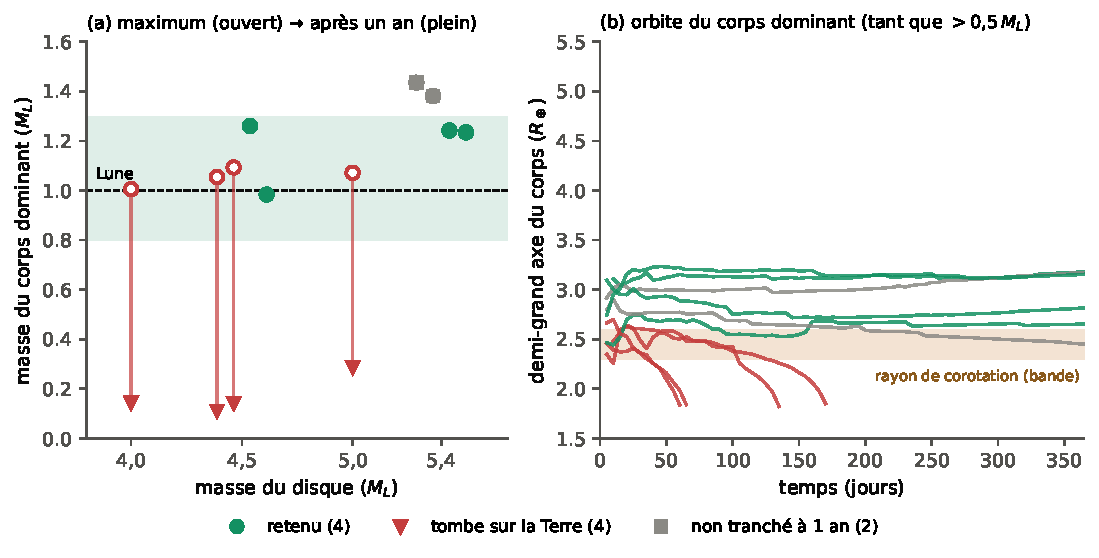
\includegraphics[width=\linewidth]{fig_synth.pdf}
\caption{Synthèse des dix réalisations calculées à $6$~h et $1{,}60\,\Rt$. (a)~Plus grande masse atteinte par le corps dominant (cercle ouvert) et sa masse après un an (symbole plein)~; la bande grise est $0{,}8$--$1{,}3\,\ML$. (b)~Demi-grand axe du corps dominant~; la bande ombrée est le rayon de corotation. Vert~: conservé. Rouge~: tombe sur la Terre entre le jour $65$ et le jour $175$. Gris~: non tranché après un an.\label{fig:synth}}
\end{figure}

Le critère retenu est simple. Une réalisation est un succès si elle forme un corps de $0{,}8$ à $1{,}3$ masse lunaire, dont le point le plus bas de l'orbite reste au-delà du rayon de corotation, sur une orbite presque circulaire dont l'inclinaison décroît, et que les marées amènent ensuite à $54$--$66\,\Rt$ en $4{,}5$ milliards d'années. Quatre réalisations satisfont les deux premières conditions après un an~: deux à $4{,}5$ et deux à $5{,}4$ masses lunaires. Elles gardent leur satellite pendant cinq ans, de $1{,}0$ à $1{,}27$ masse lunaire, sans que rien ne tombe sur la Terre après la première année. Les quatre réalisations qui perdent le corps le voient tomber entre le jour $65$ et le jour $175$ (tableau~\ref{tab:M45}). Deux ne sont pas tranchées après un an.

\begin{table}[htbp]
\centering
\caption{Les dix réalisations à $6$~h et $1{,}60\,\Rt$. Pic~: plus grande masse atteinte par le corps dominant~; $M_1$, $a_1$~: sa masse (masses lunaires) et son demi-grand axe ($\Rt$) à la fin du suivi (un an, ou cinq ans pour les réalisations conservées).\label{tab:M45}}
\small
\begin{tabular}{ccccc>{\raggedright\arraybackslash}p{6.0cm}}
\toprule
Disque ($\ML$) & graine & Pic & $M_1$ & $a_1$ & Devenir \\
\midrule
4,0 & 3 & 1,01 & 0,14 & --- & tombe sur la Terre (jour 170) \\
4,5 & 0 & 1,05 & 0,11 & --- & tombe sur la Terre (jour 65) \\
4,5 & 1 & 1,09 & 0,14 & --- & tombe sur la Terre (jour 135) \\
4,5 & 2 & 1,26 & 1,273 & 3,70 & \textbf{conservé} sur 5 ans \\
4,5 & 3 & 0,98 & 1,016 & 3,87 & \textbf{conservé} sur 5 ans \\
5,0 & 3 & 1,07 & 0,29 & --- & tombe sur la Terre (jour 60) \\
5,4 & 0 & 1,43 & 1,43 & 3,17 & non tranché à un an ($a_1>R_{\rm co}$) \\
5,4 & 1 & 1,38 & 1,38 & 2,45 & sous le rayon de corotation, non tranché \\
5,4 & 2 & 1,24 & 1,250 & 3,88 & \textbf{conservé} sur 5 ans \\
5,4 & 3 & 1,23 & 1,234 & 4,00 & \textbf{conservé} sur 5 ans \\
\bottomrule
\end{tabular}
\end{table}

\textbf{À retenir.} Plusieurs masses de disque entre $4{,}5$ et $5{,}4$ masses lunaires ont donné un satellite conservé, dans environ une réalisation sur deux. L'intervalle favorable n'est pas encore délimité~: les calculs uniques à $4{,}0$ et $5{,}0$ n'ont pas abouti à un satellite conservé, ce qui n'en exclut pas un avec d'autres graines. La valeur de $4{,}5$ masses lunaires sert de valeur de travail pour la suite parce que l'une de ses réalisations se termine par un satellite de $1{,}016$ masse lunaire. C'est une propriété de cette réalisation, non de la masse du disque.

\textbf{Le corps tient-il près de la limite de Roche\,?} Le corps dominant se tient à quelques rayons terrestres, plus près que la limite de Roche d'un liquide ($2{,}90\,\Rt$). Mais cette limite vaut pour un liquide. Un tas de gravats ou une pâte tient par sa propre pesanteur et ses contacts. On modélise le corps comme un tas de $300$ billes qui se repoussent au contact et s'attirent à distance, et l'on regarde s'il reste d'un seul tenant après $20$ tours. Sur les deux orbites issues de la phase~C, le tas reste d'un seul tenant. Le test sait pourtant détecter une destruction~: il met le tas en pièces à $1{,}6$ et $2{,}0\,\Rt$ et sa limite de désagrégation se situe entre $2{,}25$ et $2{,}5\,\Rt$, nettement plus bas que la limite fluide et plus haut que celle d'un solide rigide ($1{,}49\,\Rt$). Les orbites testées restent au-delà, avec une marge de $4\,\%$ pour la plus proche.

\subsection{Un passage plus favorable au freinage}
\label{sec:best}

Parmi les $80$ géométries dont le point le plus proche est au-dessus du disque, celle qui freine le mieux la rotation est un passage plus rasant et plus rapide~: $2{,}6\,\Rt$ et $3$~km\,s$^{-1}$, toujours rétrograde à $25^\circ$. Nous l'avons suivi jusqu'au bout, avec le même code que le passage de référence. Le tableau~\ref{tab:bestB} montre qu'il redistribue un peu moins de matière autour de la Terre ($41\,\%$ restent liés au lieu de $47\,\%$) sans changer l'inclinaison des orbites ($32^\circ$). Le freinage plus fort coûte donc un peu de redistribution, sans la supprimer.

\begin{table}[htbp]
\centering
\caption{Devenir des traceurs pour le passage de référence et pour le passage favorable au freinage (calculé, moyenne sur trois graines, $\Req=1{,}60\,\Rt$).\label{tab:bestB}}
\small
\begin{tabular}{lcccc}
\toprule
Passage & tombés sur la Terre & liés à la Terre & ont quitté la Terre & inclinaison \\
\midrule
Référence ($3{,}0\,\Rt$, $2$~km\,s$^{-1}$) & 0,210 & 0,466 & 0,325 & $31{,}5^\circ$ \\
Favorable ($2{,}6\,\Rt$, $3$~km\,s$^{-1}$) & 0,265 & 0,410 & 0,325 & $31{,}9^\circ$ \\
\bottomrule
\end{tabular}
\end{table}

On refait ensuite la phase~C avec une Terre qui tourne en $7{,}7$~h au départ, la rotation que laisserait un retrait de $0{,}21\,\LEM$. Dans chacune des cinq réalisations terminées, un corps de $0{,}71$ à $1{,}02$ masse lunaire se forme entre les jours $60$ et $230$~; aucune ne le conserve à un an. Avec cinq réalisations contre deux conservations sur cinq pour le passage de référence, la différence n'est pas mesurable~: ce petit échantillon ne permet d'affirmer ni que ce passage retient moins, ni qu'il retient autant. Le suivi de l'origine des particules montre que le corps dominant est fait de matière du disque, et le moment cinétique final ne fait que reprendre celui du départ~: la dynamique qui suit le survol ne retire presque rien. Un retrait de $0{,}21\,\LEM$ par le seul survol est d'ailleurs hors de portée d'une proto-Terre aussi condensée (section~\ref{sec:despin})~; ce calcul à $7{,}7$~h est donc un test extrême, et les retraits de $0{,}04$ à $0{,}07\,\LEM$ du bilan couplé, plus modestes, n'ont pas été testés en phase~C.

\subsection{Les marées portent le corps jusqu'à la distance lunaire}
\label{sec:migration}

La Terre tourne plus vite que le corps n'orbite~: la marée qu'elle soulève précède le corps, l'attire en avant et le pousse vers l'extérieur, en lui transférant du moment cinétique pris à la rotation de la Terre. Le corps quitte la limite de Roche en moins d'un an et s'éloigne ensuite sans s'arrêter (tableau~\ref{tab:migration}, figure~\ref{fig:migration}). Il n'atteint jamais le synchronisme avec la rotation de la Terre, et aucun cas ne retombe.

\begin{table}[htbp]
\centering
\caption{Rayon orbital ($\Rt$) du corps dominant d'après l'intégration séculaire des marées, avec une Terre qui se contracte ($\tau_c=10^5$~ans). Entre parenthèses~: période de rotation de la Terre en heures. La dernière colonne donne le rayon à $4{,}5$~Ga si la dissipation est divisée ou multipliée par $2$.\label{tab:migration}}
\footnotesize
\begin{tabular}{lcccccc}
\toprule
Satellite retenu & $10^3$ ans & $10^6$ ans & $0{,}25$ Ga & $1$ Ga & $4{,}5$ Ga & $4{,}5$ Ga, dissip. $\times(0{,}5$--$2)$ \\
\midrule
$1{,}016\,\ML$ & 8,7 (6,5) & 19,6 (5,5) & 41,9 (7,8) & 50,8 (9,1) & \textbf{62,4} (11,2) & 57--68 \\
$1{,}273\,\ML$ & 8,9 (6,9) & 19,9 (6,2) & 41,6 (10,7) & 50,0 (13,6) & \textbf{60,2} (19,9) & 55--65 \\
\bottomrule
\end{tabular}
\end{table}

\begin{figure}[htbp]
\centering
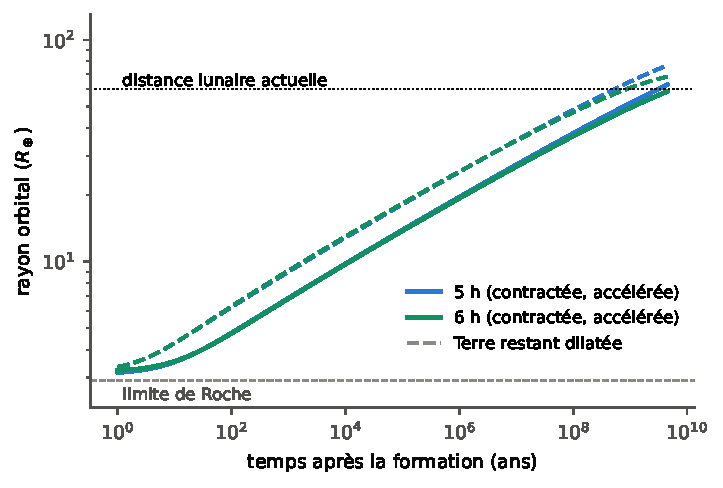
\includegraphics[width=0.82\linewidth]{fig_migration.pdf}
\caption{Rayon orbital du corps dominant sous l'effet des marées. Trait plein~: la Terre se contracte dès le départ et sa rotation s'accélère par conservation du moment cinétique. Tirets~: la Terre reste gonflée. Pointillés~: distance lunaire actuelle~; tirets gris~: limite de Roche.\label{fig:migration}}
\end{figure}

\textbf{À retenir.} Les deux satellites conservés à $4{,}5$ masses lunaires atteignent $62{,}4$ et $60{,}2\,\Rt$ en $4{,}5$ milliards d'années, pour une distance lunaire actuelle de $60{,}3\,\Rt$. L'accord est obtenu sans ajustement, avec une dissipation calibrée ailleurs, et il est robuste~: la distance varie lentement avec la dissipation. Il ne prouve pas pour autant que la Lune a suivi ce chemin~; la dissipation réelle de la Terre a varié au cours du temps. La rotation finale de la Terre (\,$11$ à $20$~h au lieu de $24$~h) est la trace de l'excès de moment cinétique, dont traite la section suivante. Si la Terre se contracte en se refroidissant, sa rotation s'accélère jusqu'à $3{,}6$--$4{,}0$~h, la rotation rapide que les modèles à impact doivent postuler \citep{CukStewart2012}, obtenue ici sans impact.

% =====================================================================
\section{Le moment cinétique de l'ensemble Terre--Lune}
\label{sec:AM}

Le moment cinétique mesure la « quantité de rotation » d'un système, celle de la Terre qui tourne sur elle-même et celle de la Lune qui tourne autour de la Terre. Il se conserve~: il peut passer de la Terre à la Lune par les marées, ou être emporté par un corps qui quitte le système, mais il ne disparaît pas. Celui de l'ensemble Terre--Lune actuel, $\LEM=3{,}5\times10^{34}$~kg\,m$^2$\,s$^{-1}$, sert d'unité dans toute cette section. C'est la question la plus difficile de toutes les théories de l'origine de la Lune, la nôtre comprise, et c'est celle sur laquelle cette version apporte le plus de nouveau.

\subsection{Ce que la Lune dit de la rotation de la Terre, lue à rebours}
\label{sec:obl}

La Lune étant une donnée, on peut intégrer à rebours le système Terre--Lune actuel jusqu'à l'époque où le satellite était à $3{,}87\,\Rt$, là où le survol le laisse. On obtient ce que la Terre devait alors avoir comme rotation et comme inclinaison d'axe. Le résultat est une condition \emph{nécessaire}, non un événement~: d'autres histoires conduisent au même présent. Le calcul inclut le couplage entre l'orbite lunaire et le renflement équatorial de la Terre, l'action du Soleil et les marées de la Lune et du Soleil.

Trois résultats ressortent (tableau~\ref{tab:retro}). Premièrement, la rotation de la Terre devait porter $0{,}79\,\LEM$ et l'orbite lunaire $0{,}21\,\LEM$, soit $0{,}994\,\LEM$ au total, quelle que soit la force de marée supposée~; cela correspond à une période de $7$~h environ. Deuxièmement, l'obliquité (l'angle de l'axe de rotation avec la normale à l'écliptique) devait être de $7$ à $13^\circ$. Troisièmement, l'orbite du satellite devait être inclinée d'environ $15^\circ$ sur l'équateur, un chiffre remarquablement stable d'un cas à l'autre. Intégré en avant depuis le satellite, le même modèle ramène une Terre qui part de $10$--$14^\circ$ aux $23{,}4^\circ$ actuels~; une Terre qui part de $0^\circ$ resterait à moins de $2^\circ$. C'est le Soleil, en ramenant l'orbite lunaire vers l'écliptique, qui fixe ce résultat.

\begin{table}[htbp]
\centering
\caption{Ce que la Lune exige, lue à rebours à $3{,}87\,\Rt$ (calculé). $F$~: facteur par lequel la marée est multipliée pour raccourcir le calcul~; $\varphi$~: phase du nœud de l'orbite lunaire, inconnue~; $\varepsilon_0$~: obliquité~; $i_{\rm eq}$~: inclinaison de l'orbite sur l'équateur.\label{tab:retro}}
\small
\begin{tabular}{lcccc}
\toprule
Cas & $\varphi$ ($^\circ$) & $\varepsilon_0$ ($^\circ$) & $i_{\rm eq}$ ($^\circ$) & Rotation de la Terre \\
\midrule
$F=10$ & 0, 90, 180, 270 & 7,3 ; 10,7 ; 12,9 ; 10,6 & 15,1 à 15,5 & $0{,}79\,\LEM$ \\
$F=4$ & 90, 180 & 6,8 ; 7,6 & 15,3 à 15,4 & $0{,}79\,\LEM$ \\
$F=25$ & 90, 180 & 13,1 ; 10,5 & 15,6 & $0{,}79\,\LEM$ \\
\bottomrule
\end{tabular}
\end{table}

Le même modèle, intégré cette fois vers l'avant depuis le satellite, répond à la question inverse~: que devient une obliquité initiale donnée au bout de $4{,}5$ milliards d'années (tableau~\ref{tab:obl})\,? L'obliquité croît pendant l'évolution, d'un facteur voisin de $2{,}4$ pour le premier satellite et de $1{,}4$ à $2{,}3$ pour le second. Les $23{,}4^\circ$ actuels sont atteints pour une obliquité initiale de $10$ à $14^\circ$, ce qui s'accorde avec les $7$ à $13^\circ$ de l'intégration à rebours. Une Terre qui partirait de $0^\circ$ finirait à moins de $2{,}3^\circ$~: dans ce modèle, une obliquité actuelle de $23^\circ$ ne peut pas venir d'une obliquité primitive de quelques degrés seulement. Le Soleil est l'ingrédient essentiel~: sans lui, l'obliquité finale serait environ deux fois plus faible et l'orbite lunaire resterait inclinée de $10$ à $32^\circ$ sur l'écliptique au lieu de moins de $4^\circ$.

\begin{table}[htbp]
\centering
\caption{Obliquité finale après $4{,}5$~Ga selon l'obliquité initiale $\varepsilon_0$ (calculé). L'intervalle couvre deux phases du n\oe ud de l'orbite lunaire.\label{tab:obl}}
\small
\begin{tabular}{rcc}
\toprule
$\varepsilon_0$ ($^\circ$) & satellite de $1{,}273\,\ML$ & satellite de $1{,}016\,\ML$ \\
\midrule
0 & 0,4 & 2,3 \\
5 & 12,0--12,7 & 7,0--11,5 \\
10 & 24,0--24,7 & 16,2--20,6 \\
15 & 35,3--35,9 & 25,2--29,4 \\
20 & 45,7--46,4 & 33,9--38,0 \\
\bottomrule
\end{tabular}
\end{table}

\textbf{À retenir.} Lue à rebours, la Lune demande une Terre qui tourne en $7$~h environ avec un axe peu incliné, au moment où le survol laisse le satellite à $3{,}9\,\Rt$. Les planètes ont été examinées par une comparaison de vitesses le long du chemin rétrodit~: la précession de l'axe reste au moins $1{,}9$ fois plus rapide que la plus grande fréquence planétaire, de sorte que leur influence est probablement faible, avec une réserve de la littérature sur un îlot de résonance pour une Terre à rotation rapide \citep{LaskarJoutelRobutel1993}. Le modèle n'a ni planètes, ni excentricité.

\textbf{Les autres planètes comme point de repère.} Les orbites des planètes sont toutes proches de l'écliptique (moins de $7{,}1^\circ$), mais leurs axes de rotation vont de $0{,}01^\circ$ à $178^\circ$~: le Soleil n'oriente pas l'axe d'une planète vers son orbite. Pour les quatre planètes internes, \citet{LaskarRobutel1993} concluent qu'aucune obliquité ne peut être considérée comme primordiale, alors que les quatre planètes géantes ont gardé la leur depuis leur formation. Des axes initiaux aléatoires sont donc la règle, et l'axe de la proto-Terre avant le survol, que la théorie ne contraint pas, n'a rien d'exceptionnel.

\subsection{L'excès de $0{,}21\,\LEM$}
\label{sec:excess}

Le système lié que le calcul produit est le suivant (tableau~\ref{tab:AM45}). Pour le satellite de $1{,}016$ masse lunaire, la rotation de la Terre, moment cinétique des corps tombés sur elle compris, porte $0{,}996\,\LEM$ et le système lié complet, orbite comprise, $1{,}208\,\LEM$. Le système Terre--Lune actuel, ramené à un satellite de même masse, porte $0{,}999\,\LEM$. Le système lié contient donc $0{,}21\,\LEM$ de trop. Les petits corps qui ont quitté le système n'en ont emporté que $0{,}017$, déjà comptés. Pour le satellite de $1{,}273$ masse lunaire, trop massif de $27\,\%$ par rapport à la Lune, l'excès n'est que de $0{,}04\,\LEM$, mais seulement parce qu'un satellite plus lourd exige plus de moment cinétique orbital à la même distance~; cela n'en fait pas une meilleure correspondance.

\begin{table}[htbp]
\centering
\caption{Bilan de moment cinétique des deux satellites conservés à $4{,}5$ masses lunaires, en unités de $\LEM$ (calculé). Le « requis » est celui d'un système Terre--Lune de même masse de satellite, à $60{,}3\,\Rt$, avec une Terre de $24$~h.\label{tab:AM45}}
\small
\begin{tabular}{lcc}
\toprule
Élément & satellite de $1{,}016\,\ML$ & satellite de $1{,}273\,\ML$ \\
\midrule
Rotation de la Terre à cinq ans & 0,996 & 0,985 \\
Système lié, total & 1,208 & 1,249 \\
Emporté par les corps qui ont quitté le système & 0,017 & 0,018 \\
Requis par le système actuel & 0,999 & 1,209 \\
\textbf{Excès} & \textbf{0,21} & \textbf{0,04} \\
Rotation de la Terre à $4{,}5$~Ga, marée lunaire seule & 11,2 h & 19,9 h \\
\bottomrule
\end{tabular}
\end{table}

\textbf{Comment situer cet excès.} Il est du même ordre que la borne de $1{,}2\,\LEM$ que \citet{Canup2014} retient pour les impacts « canoniques », et de quatre à neuf fois plus faible que celui des impacts à fort moment cinétique, dont le total est de $1{,}9$ à $2{,}8\,\LEM$ (soit $0{,}9$ à $1{,}8\,\LEM$ d'excès) et que l'évection doit alors faire retirer. Les variantes à Terre rapide doivent elles aussi évacuer du moment cinétique \citep{CukStewart2012,Tremaine2009}. Notre excès dépend de l'état de départ~: la rotation de $6$~h et le moment d'inertie de la Terre gonflée ($0{,}187\,\Mt\Req^2$). Une rotation plus rapide ou un corps plus condensé en porterait davantage.

\begin{table}[htbp]
\centering
\caption{Moment cinétique total et excès pour trois familles de chemins, en unités de $\LEM$. Les valeurs des impacts viennent de \citet{Canup2014}~; celle de cette étude est calculée ici (réalisation de $1{,}016\,\ML$).\label{tab:compAM}}
\small
\begin{tabular}{lcc}
\toprule
Chemin & Total & Excès sur $1\,\LEM$ \\
\midrule
Impact canonique (borne) & jusqu'à $1{,}2$ & jusqu'à $0{,}2$ \\
Impacts à fort moment cinétique & $1{,}9$ à $2{,}8$ & $0{,}9$ à $1{,}8$ \\
Cette étude, avant les mécanismes de retrait & $1{,}21$ & $0{,}21$ \\
\bottomrule
\end{tabular}
\end{table}

\subsection{Ce que la planète~$B$ retire à la rotation}
\label{sec:despin}

La planète~$B$ ne repart pas les mains vides. En passant, elle soulève sur la proto-Terre un renflement de marée. Ce renflement est en retard sur la direction de la planète~$B$ parce que la matière ne répond pas instantanément~; l'attraction de la planète~$B$ sur ce renflement décalé freine la rotation de la Terre, la chaleur correspondante est dissipée dans la Terre, et le moment cinétique perdu par la rotation passe dans le mouvement de la planète~$B$. Le survol étant rétrograde, la surface de la Terre défile sous la planète~$B$ à la vitesse relative $\Omega_\oplus+|\dot\phi_B|$, toujours positive~: \emph{le signe du freinage est donc certain}. Sa grandeur dépend de la quantité de marée que la Terre transforme en chaleur.

\textbf{Un corps mou, ni liquide ni rigide.} Un liquide suit la marée sans frotter~; un solide froid se déforme à peine~; la dissipation est la plus forte entre les deux, pour une matière molle. C'est le cas de la proto-Terre de cette théorie, et le passage de la planète~$B$ ne change pas ce caractère. Nous avons calculé jusqu'où va cette dissipation avec une rhéologie de Maxwell, qui décrit une matière élastique pour les marées rapides et visqueuse pour les marées lentes, d'abord pour un corps uniforme, puis pour des corps stratifiés (un noyau liquide, un manteau pâteux, une enveloppe gonflée). Trois résultats ressortent.

\begin{enumerate}[leftmargin=1.6em,itemsep=2pt]
\item \emph{La matière qui dissipe le mieux est une pâte épaisse}, de viscosité de l'ordre de $10^{12}$~Pa\,s (environ un million de milliards de fois celle de l'eau), pas un liquide. Une enveloppe liquide ne dissipe presque rien. La dissipation doit donc se produire dans la matière molle, à travers toute l'épaisseur du corps.
\item \emph{Le fait que la marée monte puis retombe pendant le survol ne change pas le résultat}~: un calcul qui suit la marée instant par instant donne le même freinage à $2\,\%$ près, parce que l'effet se concentre autour du point le plus proche et que la pâte réagit en quelques minutes.
\item \emph{La dissipation maximale dépend de la condensation du corps.} Plus la Terre est condensée vers le centre, moins elle se déforme et moins elle dissipe (tableau~\ref{tab:interieur}).
\end{enumerate}

La dissipation maximale d'un corps uniforme croît avec sa rigidité jusqu'à un plateau (tableau~\ref{tab:rigidite}). Elle est presque nulle pour un corps presque liquide ($0{,}013$ pour $0{,}1$~GPa), atteint $0{,}26$ vers $3$~GPa, ce qui suffit au passage favorable, et $0{,}48$ à $10$~GPa, ce qui suffit aux deux passages. Il faut donc une matière qui ait un peu de rigidité, c'est-à-dire une pâte et non un liquide.

\begin{table}[htbp]
\centering
\caption{Dissipation maximale $k_2/Q$ d'un corps uniforme de rhéologie de Maxwell, selon sa rigidité (calculé, viscosité la plus favorable).\label{tab:rigidite}}
\small
\begin{tabular}{cccccc}
\toprule
Rigidité (GPa) & $0{,}1$ & $1$ & $3$ & $10$ & $70$ \\
\midrule
$k_2/Q$ maximal & 0,013 & 0,115 & 0,263 & 0,483 & 0,695 \\
\bottomrule
\end{tabular}
\end{table}

\begin{table}[htbp]
\centering
\caption{Freinage maximal que la rhéologie de Maxwell permet, en $\LEM$, pour quelques corps stratifiés dont le moment d'inertie réduit $C/(MR^2)$ varie (calculé). « Passage de référence »~: distance $3{,}0\,\Rt$, $2$~km\,s$^{-1}$. « Passage favorable »~: $2{,}6\,\Rt$, $3$~km\,s$^{-1}$. La monographie emploie $C/(MR^2)=0{,}187$ pour la proto-Terre gonflée.\label{tab:interieur}}
\small
\begin{tabular}{lccc}
\toprule
Corps & $C/(MR^2)$ & passage de référence & passage favorable \\
\midrule
Noyau et manteau, sans enveloppe & 0,30 & 0,21 & 0,38 \\
Enveloppe de $0{,}22$ masse terrestre & 0,20 & 0,05 & 0,09 \\
Enveloppe de $0{,}17$ (valeur de la monographie) & 0,19 & \textbf{0,04} & \textbf{0,07} \\
Enveloppe de $0{,}50$ & 0,29 & 0,18 & 0,33 \\
\bottomrule
\end{tabular}
\end{table}

\textbf{À retenir.} Pour une proto-Terre aussi condensée que dans cette étude, un corps mou retire au plus $0{,}04\,\LEM$ avec le passage de référence et $0{,}07\,\LEM$ avec le passage le plus favorable~; avec la marée utilisée dans la monographie, le retrait est plus modeste encore, de $0{,}012$ à $0{,}027\,\LEM$. Ce n'est donc \emph{pas} le seul mécanisme capable de fermer le bilan~; c'est une contribution réelle, de l'ordre de $0{,}01$ à $0{,}07\,\LEM$ selon la dissipation de la matière molle. Un corps nettement moins condensé retirerait davantage, mais il porterait aussi plus de moment cinétique à période égale, et ce second cas n'a pas été recalculé.

\textbf{L'axe.} Le même survol fait basculer l'axe de la Terre sans changer le moment cinétique de la rotation. La bascule dépend de l'aplatissement de la proto-Terre, qui n'est pas connu pour un corps chaud~: elle vaut de $2^\circ$ à $30^\circ$ selon cet aplatissement. L'intervalle de $7$ à $13^\circ$ que demande la Lune est à l'intérieur de cette plage, ce qui est une cohérence d'ordres de grandeur et non un test. L'axe ne devient pas parallèle à l'orbite de la planète~$B$. Un écart reste non résolu~: l'aplatissement qui donne la bascule de $10^\circ$ n'est pas celui du corps stratifié le plus proche de la monographie, et un modèle intérieur unique qui donnerait ensemble moment d'inertie, aplatissement, dissipation et rotation n'est pas construit.

\subsection{Les autres mécanismes, pris un à un}
\label{sec:puits}

Trois autres mécanismes retirent du moment cinétique, que nous avons d'abord testés séparément.

\textbf{La marée solaire sur la Terre.} Le Soleil soulève lui aussi une marée sur la Terre, qui freine sa rotation, le moment cinétique perdu passant à l'orbite de la Terre autour du Soleil. Avec la même dissipation que la marée lunaire, elle retire $0{,}017\,\LEM$ en $4{,}5$ milliards d'années, soit environ $8\,\%$ de l'excès.

\textbf{Les corps qui quittent le système.} Les petits corps non liés emportent $0{,}017$ à $0{,}018\,\LEM$. Ils sont déjà comptés dans le bilan du tableau~\ref{tab:AM45}.

\textbf{La résonance d'évection.} Quand le satellite est encore proche de la Terre, la précession de son orbite peut se synchroniser avec la période de révolution de la Terre autour du Soleil. Le satellite est alors piégé un temps dans une résonance où son orbite s'allonge fortement~; pendant ce piégeage, la gravité du Soleil prélève du moment cinétique sur l'ensemble Terre--Lune au profit de l'orbite de la Terre autour du Soleil, et le système en sort allégé \citep{CukStewart2012,WardCanupRufu2020,RufuCanup2020}. Nous l'avons étudiée avec un modèle séculaire plan (annexe~\ref{app:evec}). Avec une marée terrestre d'au moins $0{,}1$ fois la référence, elle retire au plus $0{,}03\,\LEM$~; des valeurs plus grandes, jusqu'à $0{,}06\,\LEM$, ne sont obtenues qu'avec des marées $100$ à $1000$ fois plus faibles, ce qui laisserait le satellite à une vingtaine de rayons terrestres seulement après $4{,}5$ milliards d'années. Ces valeurs sont celles du mécanisme pris isolément~; la durée de contraction de la proto-Terre, qui commande le rendement, n'intervient que dans le bilan couplé (section~\ref{sec:couple}), où le retrait moyen atteint $0{,}16\,\LEM$ pour $\tau_c=2\times10^6$~ans, et la durée des captures est donnée à l'annexe~\ref{app:trois}.

\textbf{À retenir.} Pris séparément, aucun de ces mécanismes ne retire $0{,}21\,\LEM$. La marée solaire en retire $0{,}017$, le freinage par la planète~$B$ de $0{,}01$ à $0{,}07$, l'évection jusqu'à $0{,}03$ pour une marée terrestre usuelle. Mais ils ne s'additionnent pas simplement, parce qu'ils agissent sur le même système, l'un après l'autre, et que chacun modifie les conditions du suivant. Le bilan doit donc être calculé sur une seule trajectoire.

\subsection{Les mécanismes agissent ensemble~: le bilan couplé}
\label{sec:couple}

Les trois mécanismes se suivent dans le temps et se modifient l'un l'autre. Le freinage par la planète~$B$ a lieu en quelques heures, et il fixe la rotation avec laquelle la Terre aborde la suite. L'évection se joue ensuite pendant des milliers à des millions d'années, tant que le satellite est proche~; elle dépend de la rotation de la Terre, de sa marée et de son rayon, qui diminue pendant que la proto-Terre se refroidit. La marée lunaire et la marée solaire finissent le travail pendant des milliards d'années. On ne peut donc pas additionner les retraits calculés séparément. Nous avons construit un calcul qui enchaîne les trois étapes sur \emph{une seule trajectoire}, à partir du satellite conservé de $1{,}016$ masse lunaire.

\textbf{Les précisions qui fixent le cadre.} Trois points, qui sont des choix de la théorie, déterminent ce calcul.
\begin{itemize}[leftmargin=1.6em,itemsep=2pt]
\item La proto-Terre est un corps \emph{mou, jamais liquide}. Le passage de la planète~$B$ ne change en rien ce caractère.
\item La planète~$B$ emporte malgré tout un peu de moment cinétique de rotation, comme on l'a vu à la section~\ref{sec:despin}. Nous la représentons par un retrait $\Delta L_B$, pris à $0$, $0{,}04$ ou $0{,}07\,\LEM$ (et de $0{,}05$ à $0{,}20\,\LEM$ dans un premier balayage). Les valeurs $0{,}04$ et $0{,}07$ sont le maximum que permet un corps mou aussi condensé que dans cette étude, pour le passage de référence et pour le passage le plus favorable.
\item La marée d'un corps mou n'est pas celle d'un corps solide, ce qui explique une faiblesse au début de l'histoire. Nous traduisons cela par une marée terrestre \emph{précoce}, pendant le passage dans l'évection, égale à une petite fraction de la marée de référence ($0{,}03$ à $0{,}3\,\%$). Cette faiblesse est \emph{posée} par le calcul, non démontrée~: la dissipation d'un corps mou dépend de sa viscosité, que nous n'avons pas calculée pour cette phase. C'est une condition à établir.
\end{itemize}

\textbf{Le calcul.} La rotation de départ est celle de la section~\ref{sec:excess} diminuée de $\Delta L_B$. La proto-Terre se contracte de $1{,}60\,\Rt$ à $1\,\Rt$ avec une durée caractéristique $\tau_c$, que le calcul fait varier de cent mille à quelques millions d'années. Le satellite entre dans la résonance d'évection, y est piégé ou non selon sa phase d'arrivée, puis, quand il en sort, la marée lunaire et la marée solaire le portent jusqu'à $4{,}5$ milliards d'années. La marée des derniers milliards d'années est \emph{ajustée} de façon que la distance finale soit exactement de $60{,}3\,\Rt$~; elle n'est pas imposée, car la dissipation réelle de la Terre a varié au cours du temps. Le calcul n'est d'ailleurs pas fait pour reproduire la fuite actuelle de la Lune ($3{,}8$~cm par an, contre $1{,}15$ dans le modèle à la fin)~: il transfère de la rotation vers l'orbite sans rien retirer, de sorte que l'excès final dépend peu de ce détail. Le moment cinétique total est conservé à $10^{-6}\,\LEM$ près à chaque étape. Sans évection ni freinage, le calcul retrouve les valeurs de la section~\ref{sec:puits} ($1{,}191\,\LEM$ et $62{,}2\,\Rt$ avec la marée solaire seule).

\textbf{Ce que le calcul donne, et comment nous le lisons.} Le résultat de chaque trajectoire est l'\emph{excès final}~: le moment cinétique du système à $4{,}5$ milliards d'années, moins celui qu'exige la Lune ($0{,}999\,\LEM$). La cible est fixe~; seul l'excès de départ à éliminer varie d'une réalisation à l'autre.
\[
\Delta L_{\rm final}=L_{\rm calculé}-L_{\rm cible},
\qquad
\text{bilan fermé}\iff|\Delta L_{\rm final}|\le\varepsilon .
\]
Un excès final nul serait une fermeture parfaite~; un excès de $+0{,}10\,\LEM$ signifie que le système en garde trop, un excès de $-0{,}10\,\LEM$ qu'il en a perdu trop. Aucun calcul ne tombe exactement sur zéro, il faut donc se donner une tolérance. Nous appelons \emph{fenêtre} sa demi-largeur $\varepsilon$~: avec $\varepsilon=0{,}05\,\LEM$, le bilan est dit fermé si l'excès final est compris entre $-0{,}05$ et $+0{,}05\,\LEM$. Un excès trop négatif ne ferme donc pas le bilan, même si le mécanisme a retiré assez de moment cinétique~: la trajectoire n'aboutit pas à la fermeture. Il en va de même pour une trajectoire où la Lune est perdue.

Nous ne fixons pas une fenêtre unique, parce qu'aucune n'est imposée par la physique du problème. Nous en donnons quatre, de $\pm0{,}03$ à $\pm0{,}10\,\LEM$.
\begin{itemize}[leftmargin=1.6em,itemsep=2pt]
\item $\pm0{,}03\,\LEM$ est un critère \emph{strict} de comparaison. Il est du même ordre que l'écart d'une trajectoire à l'autre, qui vient de différences entre trajectoires du modèle (phase d'arrivée dans la résonance, paramètres), non nécessairement d'une erreur de calcul.
\item $\pm0{,}08\,\LEM$ est un critère \emph{exploratoire large}. Il tient compte de ce que l'excès de départ dépend de la réalisation~: il vaut $0{,}21\,\LEM$ pour celle que nous suivons et $0{,}04\,\LEM$ pour une autre, soit $0{,}17\,\LEM$ d'écart, dont la moitié est de l'ordre de $0{,}08\,\LEM$. C'est une échelle de sensibilité entre deux réalisations, non une marge d'erreur statistique~; nous ne la présentons pas comme une tolérance déduite de la physique.
\end{itemize}
Les résultats sont donnés sous forme de \emph{parts de trajectoires} de la grille de paramètres explorée (marée précoce, dissipation lunaire, phase d'arrivée, durée de contraction). Ces parts ne sont pas des probabilités. Avec $36$ trajectoires par ligne, une trajectoire pèse environ $2{,}8$ points de pourcentage~: une différence d'un ou deux points de grille n'a pas de portée statistique. Quatre résultats ressortent.

\paragraph{1. La durée de contraction commande le rendement de l'évection.} Pour une proto-Terre qui se contracte vite ($\tau_c\le2\times10^5$ ans), l'évection ne retire en moyenne que $0{,}03$ à $0{,}05\,\LEM$ et le bilan ne se ferme à $\pm0{,}03\,\LEM$ dans aucune trajectoire sans freinage de la planète~$B$. Pour une contraction plus lente, de $3\times10^5$ à $2\times10^6$ ans, elle retire en moyenne de $0{,}04$ à $0{,}16\,\LEM$ selon le cas, avec des trajectoires qui atteignent $0{,}30\,\LEM$ (tableau~\ref{tab:couple}). Le satellite reste conservé, sauf pour les contractions les plus longues, où il est perdu sur la Terre dans une partie des trajectoires. Les durées de capture dans la grille vont de $0{,}5$ à $435$ milliers d'ans (annexe~\ref{app:trois})~; la sensibilité des parts de fermeture au rendement de l'évection et à l'état de départ est donnée à l'annexe~\ref{app:ferm}.

\begin{table}[htbp]\centering\footnotesize\setlength{\tabcolsep}{3.6pt}
\caption{Bilan couplé, trajectoire par trajectoire~: pour chaque retrait $\Delta L_B$ par la planète~$B$ et chaque durée de contraction $\tau_c$ (en ans), moyenne et maximum du retrait par l'évection, excès final (moyenne, minimum, maximum), part des trajectoires dont l'excès final est compris entre $-\varepsilon$ et $+\varepsilon$ pour quatre fenêtres, et nombre de trajectoires où la Lune est perdue (elles ne ferment pas le bilan). Chaque ligne regroupe $36$ trajectoires (trois marées précoces de $0{,}03$ à $0{,}3\,\%$, trois dissipations lunaires, quatre phases)~; une trajectoire représente donc environ $2{,}8$ points de pourcentage. Les excès sont en unités de $\LEM$.\label{tab:couple}}
\begin{tabular}{ccccccccc}\toprule
$\Delta L_B$ & $\tau_c$ & évection moy. (max.) & excès final moy. [min.\,; max.] & $\varepsilon{=}0{,}03$ & $0{,}05$ & $0{,}08$ & $0{,}10$ & Lune perdue \\
\midrule
0,00 & 100~k & 0,03 (0,12) & 0,16 [0,07\,; 0,19] & 0\,\% & 0\,\% & 3\,\% & 6\,\% & 0/36 \\
0,00 & 200~k & 0,05 (0,14) & 0,15 [0,06\,; 0,19] & 0\,\% & 0\,\% & 14\,\% & 17\,\% & 0/36 \\
0,00 & 300~k & 0,08 (0,20) & 0,11 [0,00\,; 0,19] & 17\,\% & 19\,\% & 33\,\% & 39\,\% & 0/36 \\
0,00 & 500~k & 0,10 (0,25) & 0,09 [$-$0,06\,; 0,19] & 11\,\% & 25\,\% & 44\,\% & 50\,\% & 0/36 \\
0,00 & 1~M & 0,13 (0,30) & 0,06 [$-$0,11\,; 0,19] & 25\,\% & 25\,\% & 39\,\% & 58\,\% & 0/36 \\
0,00 & 2~M & 0,16 (0,29) & 0,03 [$-$0,10\,; 0,19] & 6\,\% & 28\,\% & 50\,\% & 64\,\% & 4/36 \\
\addlinespace
0,04 & 100~k & 0,03 (0,09) & 0,13 [0,06\,; 0,15] & 0\,\% & 0\,\% & 8\,\% & 19\,\% & 0/36 \\
0,04 & 200~k & 0,05 (0,15) & 0,11 [0,00\,; 0,15] & 8\,\% & 14\,\% & 25\,\% & 39\,\% & 0/36 \\
0,04 & 300~k & 0,07 (0,19) & 0,08 [$-$0,03\,; 0,15] & 17\,\% & 31\,\% & 47\,\% & 56\,\% & 0/36 \\
0,04 & 500~k & 0,10 (0,29) & 0,05 [$-$0,14\,; 0,15] & 6\,\% & 31\,\% & 50\,\% & 75\,\% & 0/36 \\
0,04 & 1~M & 0,11 (0,28) & 0,04 [$-$0,12\,; 0,15] & 22\,\% & 25\,\% & 50\,\% & 56\,\% & 2/36 \\
0,04 & 2~M & 0,12 (0,28) & 0,03 [$-$0,13\,; 0,15] & 19\,\% & 22\,\% & 33\,\% & 47\,\% & 6/36 \\
\addlinespace
0,07 & 100~k & 0,02 (0,10) & 0,10 [0,02\,; 0,12] & 3\,\% & 6\,\% & 17\,\% & 33\,\% & 0/36 \\
0,07 & 200~k & 0,05 (0,14) & 0,07 [$-$0,01\,; 0,12] & 22\,\% & 28\,\% & 50\,\% & 56\,\% & 0/36 \\
0,07 & 300~k & 0,04 (0,16) & 0,08 [$-$0,03\,; 0,12] & 8\,\% & 36\,\% & 44\,\% & 56\,\% & 0/36 \\
0,07 & 500~k & 0,08 (0,21) & 0,04 [$-$0,08\,; 0,12] & 22\,\% & 31\,\% & 64\,\% & 69\,\% & 1/36 \\
0,07 & 1~M & 0,10 (0,25) & 0,02 [$-$0,13\,; 0,12] & 8\,\% & 33\,\% & 44\,\% & 50\,\% & 2/36 \\
0,07 & 2~M & 0,09 (0,22) & 0,03 [$-$0,10\,; 0,12] & 19\,\% & 19\,\% & 31\,\% & 31\,\% & 11/36 \\
\bottomrule\end{tabular}\end{table}

\paragraph{2. Le bilan se ferme dans une part notable des trajectoires, et la planète~$B$ y aide modestement.} Le tableau~\ref{tab:fenetres} donne la part des trajectoires qui ferment le bilan, pour les contractions de $5\times10^5$ à $10^6$ ans et pour chaque fenêtre.

\begin{table}[htbp]\centering\small
\caption{Part des trajectoires qui ferment le bilan, selon la fenêtre $\varepsilon$ (le bilan est fermé si l'excès final est compris entre $-\varepsilon$ et $+\varepsilon$, en unités de $\LEM$). Durées de contraction de $5\times10^5$ à $10^6$ ans~; chaque case regroupe $36$ trajectoires par durée, la fourchette donnant les deux durées. Une Lune perdue compte parmi les trajectoires qui n'aboutissent pas à la fermeture. Ce sont des parts d'une grille de paramètres, non des probabilités~; la fenêtre $\pm0{,}03$ est un critère strict de comparaison, la fenêtre $\pm0{,}08$ un critère exploratoire large.\label{tab:fenetres}}
\begin{tabular}{cccc}\toprule
Fenêtre $\varepsilon$ & sans freinage par $B$ & $B$ retire $0{,}04\,\LEM$ & $B$ retire $0{,}07\,\LEM$ \\
\midrule
$\pm0{,}03$ (strict) & 11\,--\,25\,\% & 6\,--\,22\,\% & 8\,--\,22\,\% \\
$\pm0{,}05$ & 25\,\% & 25\,--\,31\,\% & 31\,--\,33\,\% \\
$\pm0{,}08$ (large) & 39\,--\,44\,\% & 50\,\% & 44\,--\,64\,\% \\
$\pm0{,}10$ & 50\,--\,58\,\% & 56\,--\,75\,\% & 50\,--\,69\,\% \\
\bottomrule\end{tabular}\end{table}

La lecture est la suivante. À $\pm0{,}05\,\LEM$, le bilan se ferme dans environ un quart à un tiers des trajectoires (de $25$ à $33\,\%$), et à $\pm0{,}08\,\LEM$ dans environ deux cinquièmes à deux tiers (de $39$ à $64\,\%$). Au critère strict de $\pm0{,}03\,\LEM$, la part est de $6$ à $25\,\%$. Le freinage par la planète~$B$ ne produit pas une amélioration à toutes les fenêtres~: à $\pm0{,}03\,\LEM$, les parts avec et sans freinage se recouvrent. Il augmente en revanche la part des fenêtres intermédiaires et larges, surtout pour la contraction de $5\times10^5$ ans, où la part à $\pm0{,}08\,\LEM$ passe de $44\,\%$ sans freinage à $50\,\%$ avec $0{,}04\,\LEM$ et à $64\,\%$ avec $0{,}07\,\LEM$. C'est une tendance, à l'échelle de la grille. Chaque $0{,}01\,\LEM$ retiré par la planète~$B$ est autant que l'évection n'a plus à retirer, ce qui explique cette tendance (figures~\ref{fig:etapes}, \ref{fig:tauc} et~\ref{fig:carte}).

Une grandeur voisine ne doit pas être confondue avec la fermeture~: dans $25$ à $47\,\%$ des trajectoires de ces durées, le mécanisme retire \emph{au moins} le niveau requis (excès final inférieur ou égal à $+0{,}03\,\LEM$, quelle que soit sa valeur négative). C'est une mesure de capacité de retrait, qui compte aussi les trajectoires qui retirent trop. Pour les contractions les plus longues, le satellite est perdu sur la Terre dans une partie des trajectoires ($11$ sur $36$ à $2\times10^6$ ans avec $0{,}07\,\LEM$)~: ces trajectoires n'aboutissent pas à la fermeture, ce qui borne la fenêtre par le haut.

\begin{figure}[htbp]
\centering
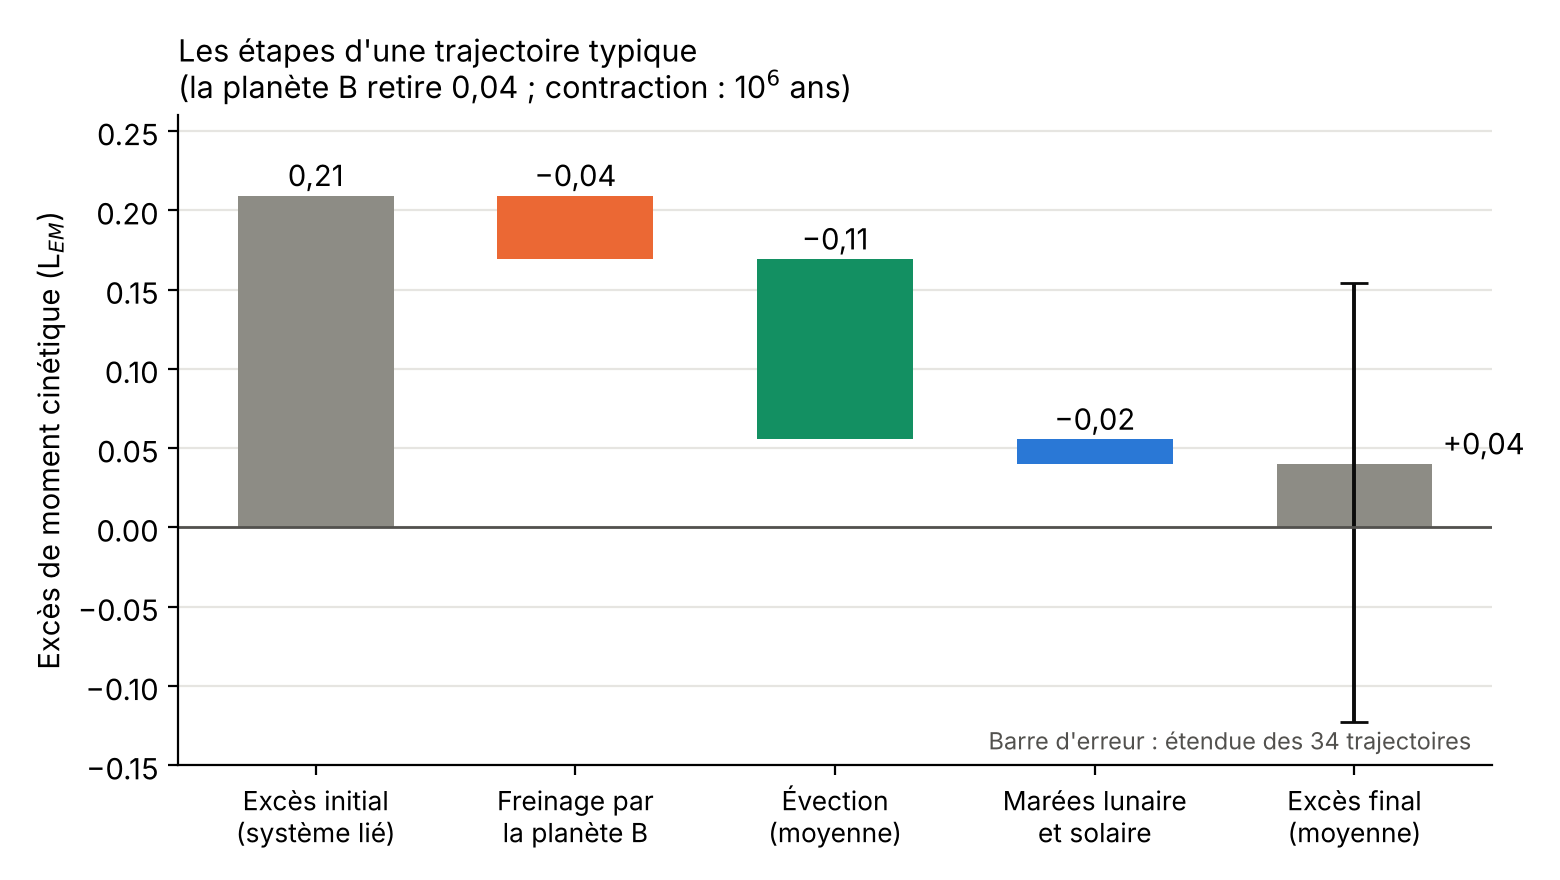
\includegraphics[width=0.78\linewidth]{fig_etapes_fr.png}
\caption{Les étapes d'une trajectoire typique, en moyenne sur les $34$ trajectoires où le satellite est conservé (retrait de $0{,}04\,\LEM$ par la planète~$B$, contraction de $10^6$ ans)~: l'excès initial de $0{,}21\,\LEM$ est réduit par le freinage de la planète~$B$, par l'évection, puis par les marées. La barre d'erreur donne l'étendue de l'excès final, de $-0{,}12$ à $+0{,}15\,\LEM$.\label{fig:etapes}}
\end{figure}

\begin{figure}[htbp]
\centering
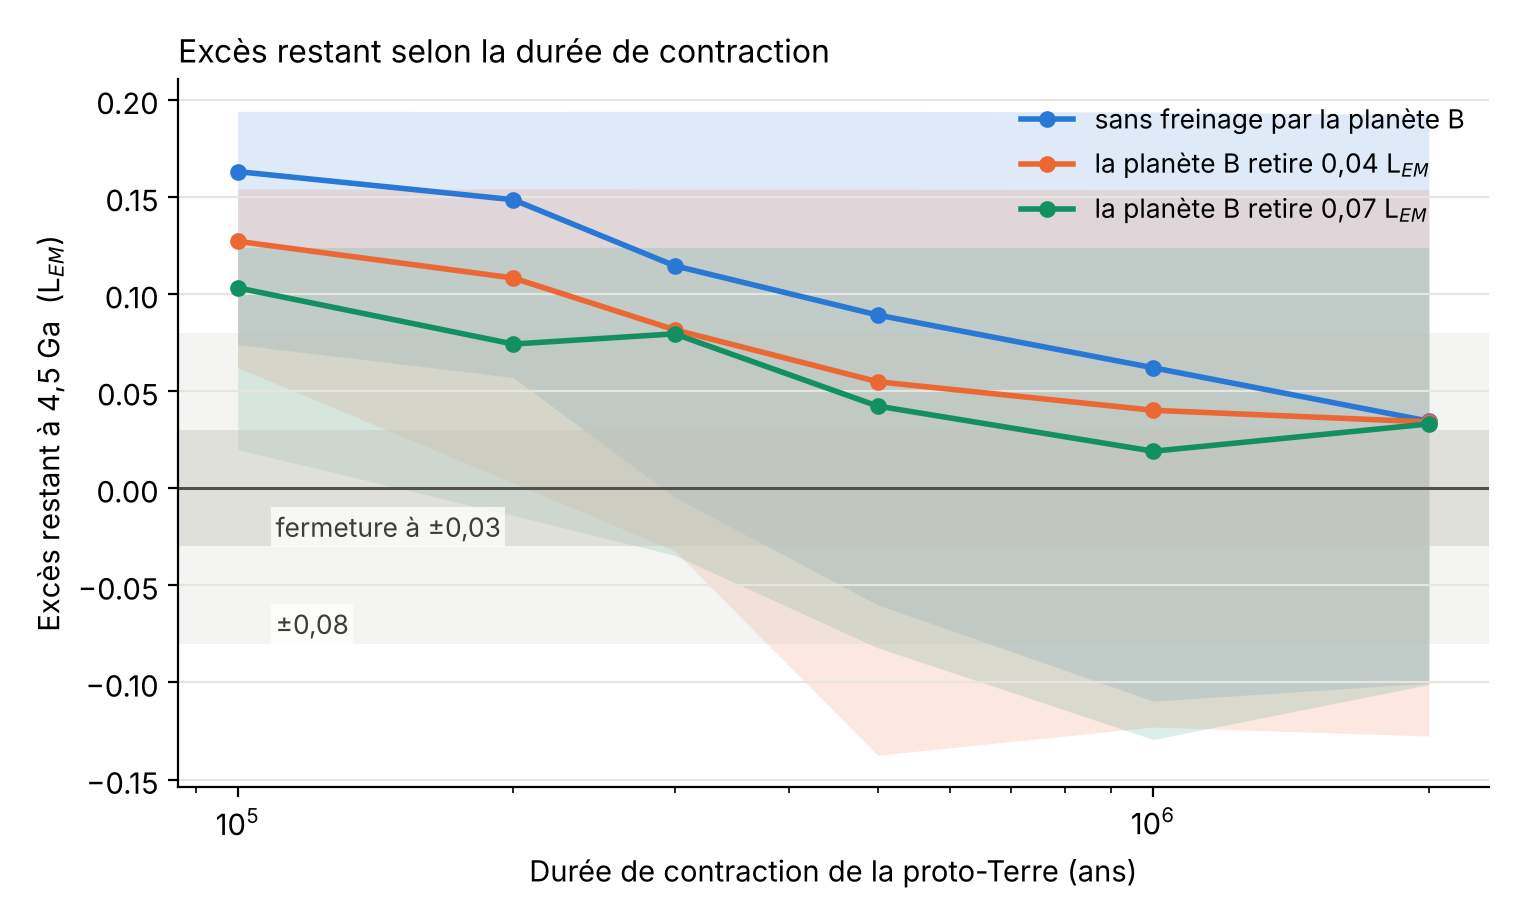
\includegraphics[width=0.78\linewidth]{fig_tauc_fr.png}
\caption{Excès de moment cinétique restant à $4{,}5$ milliards d'années, selon la durée de contraction de la proto-Terre. La ligne est la moyenne, la zone colorée l'étendue des trajectoires~; la bande grise foncée est la fenêtre stricte ($\pm0{,}03\,\LEM$), la bande claire la fenêtre exploratoire large ($\pm0{,}08\,\LEM$). Un excès négatif signifie que la trajectoire a retiré plus que nécessaire.\label{fig:tauc}}
\end{figure}

\begin{figure}[htbp]
\centering
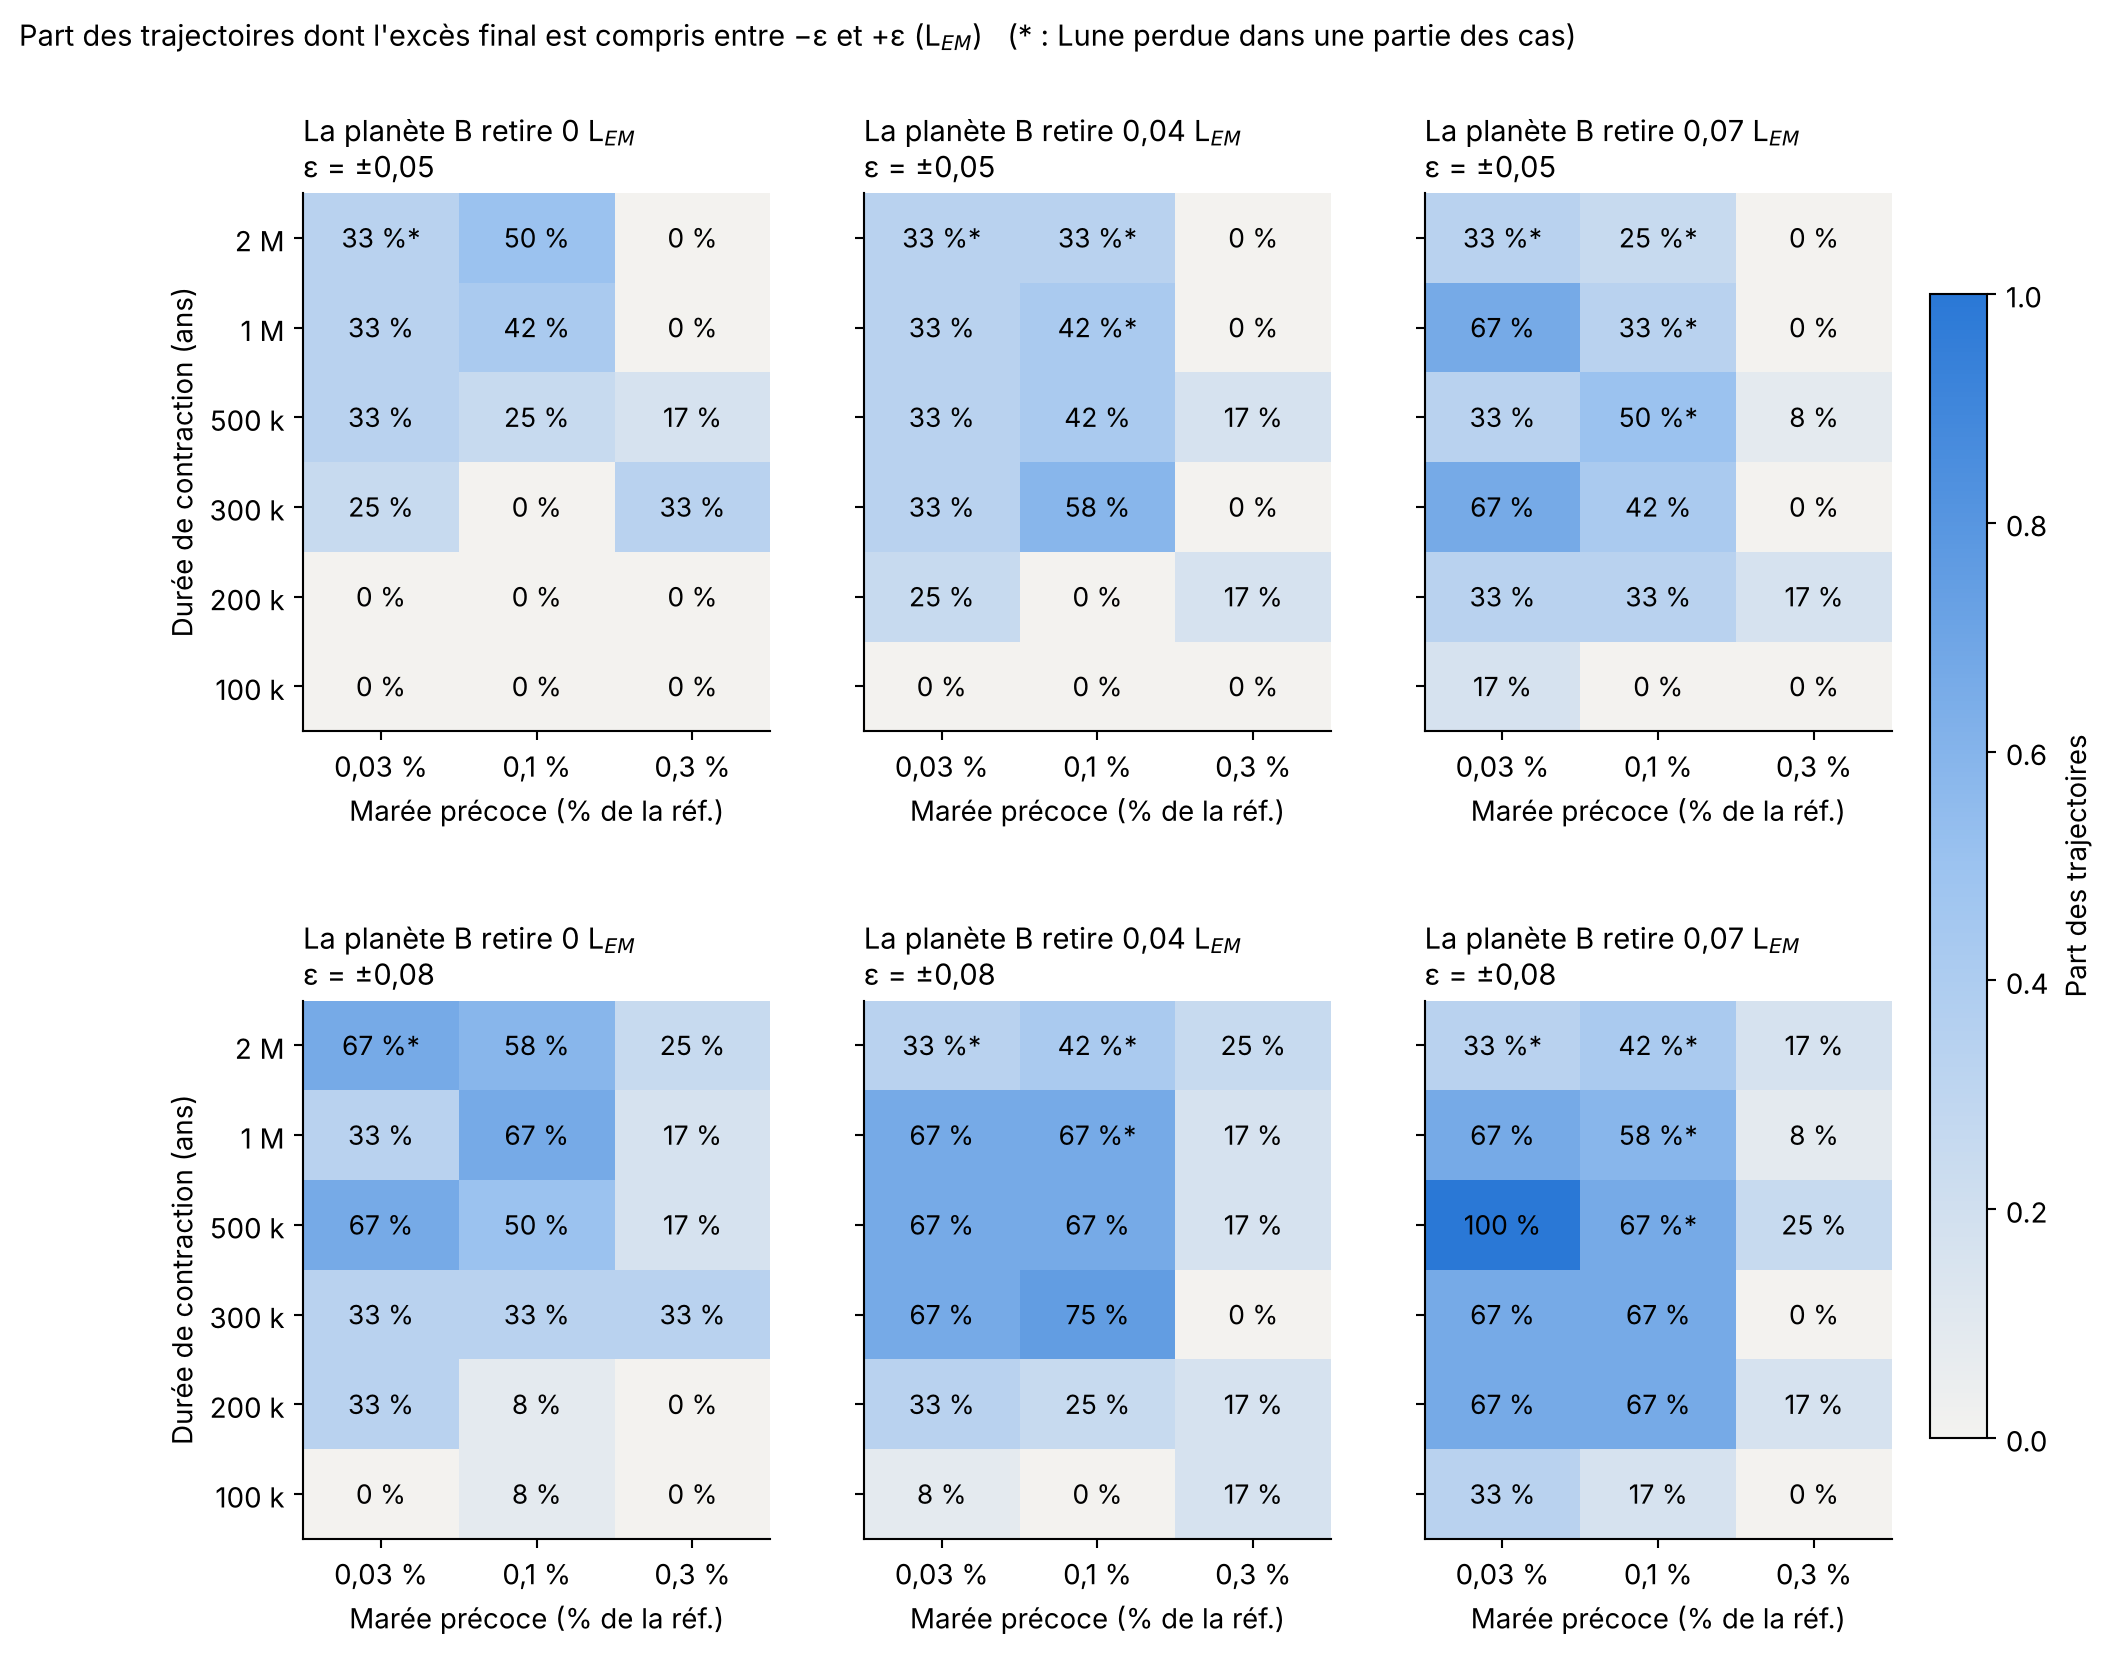
\includegraphics[width=\linewidth]{fig_map_fr.png}
\caption{Part des trajectoires dont l'excès final est compris entre $-\varepsilon$ et $+\varepsilon$, pour $\varepsilon=0{,}05\,\LEM$ (en haut) et $0{,}08\,\LEM$ (en bas), en fonction de la durée de contraction de la proto-Terre et de la marée terrestre précoce, pour trois valeurs du retrait par la planète~$B$. Chaque case regroupe les trajectoires de trois dissipations lunaires et de quatre phases d'arrivée dans la résonance (douze trajectoires, soit environ $8$ points de pourcentage par trajectoire). Un astérisque indique que la Lune est perdue dans une partie des trajectoires de la case.\label{fig:carte}}
\end{figure}

\paragraph{3. Deux conditions déterminent la fenêtre.} La fermeture exige (i)~une marée terrestre précoce faible, de $0{,}03$ à $0{,}1\,\%$ de la référence (à $0{,}3\,\%$ la fermeture devient rare, et à $1\,\%$ l'évection ne retire presque rien, moins de $0{,}02\,\LEM$ en moyenne)~; et (ii)~une contraction lente de la proto-Terre, de $2$ à $3\times10^5$ ans au moins. Ces deux conditions sont énoncées, non démontrées. La première est cohérente avec ce que l'on attend d'un corps mou, dont la marée est faible au début~; mais, la viscosité de la matière n'étant pas calculée pour cette phase, elle reste à établir. La seconde est de l'ordre des durées de refroidissement discutées pour les océans de magma sous une enveloppe de vapeur \citep{ElkinsTanton2012,Hamano2013}~; elle reste elle aussi une condition.

\paragraph{4. La dispersion d'une trajectoire à l'autre est réelle.} Le rendement de l'évection varie de $\pm0{,}01$ à $\pm0{,}03\,\LEM$ d'une trajectoire à l'autre. Cette dispersion résulte de différences entre trajectoires du modèle (phase d'arrivée dans la résonance, paramètres), non nécessairement d'une erreur de calcul. Seule la distribution des résultats a un sens, et c'est pourquoi nous la donnons sous forme de parts de trajectoires et d'étendues, non de valeurs uniques.

\textbf{Limites.} Quatre limites doivent rester présentes à l'esprit. Le modèle est plan et séculaire~: il traite la Terre, la Lune et le Soleil sans mouvement hors du plan et sans intégration à trois corps. L'état du satellite après le survol est celui de la réalisation retenue, seule la rotation de la Terre étant réduite~; la phase~C n'a pas été refaite avec cette rotation, et la conservation du satellite dépend du rayon de corotation, donc de la rotation retenue. Les rendements d'évection obtenus, de $0{,}1$ à $0{,}3\,\LEM$ dans les trajectoires les plus favorables, sont supérieurs à ceux que donne la littérature, de quelques pour cent à une dizaine de pour cent du moment cinétique du système \citep{WardCanupRufu2020,RufuCanup2020}~; ils dépendent des deux conditions ci-dessus, et c'est précisément pourquoi celles-ci doivent être établies. Enfin, les durées de contraction et les marées précoces sont des paramètres, non des prédictions.

\textbf{À retenir.} Dans le modèle séculaire couplé, le freinage par la planète~$B$ (de $0$ à $0{,}07\,\LEM$), l'évection et la marée solaire permettent d'obtenir un excès final compris entre $-0{,}05$ et $+0{,}05\,\LEM$ dans environ $25$ à $33\,\%$ des trajectoires explorées, et entre $-0{,}08$ et $+0{,}08\,\LEM$ dans environ $39$ à $64\,\%$ d'entre elles, pour des durées de contraction de $5\times10^5$ à $10^6$ ans. Ces résultats dépendent notamment d'une faible dissipation terrestre précoce et d'une contraction suffisamment lente de la proto-Terre. Les pourcentages caractérisent la grille de paramètres étudiée, non une probabilité de formation de la Lune. C'est la piste que propose la théorie pour l'excès de moment cinétique~: elle est cohérente avec une proto-Terre molle qui dissipe peu au début et dont le refroidissement prend du temps, mais elle ne le démontre pas.

\subsection{Les pistes pour l'excès}
\label{sec:pistes}

\begin{encadre}{Pistes pour l'excès de moment cinétique}
\small
\textbf{1. Le freinage par la planète~$B$} retire de $0{,}01$ à $0{,}07\,\LEM$ à la rotation, selon la dissipation de la matière molle~; il est certain en signe, et d'autant plus grand que la proto-Terre est moins condensée.

\smallskip\noindent\textbf{2. La marée solaire} retire $0{,}017\,\LEM$ en $4{,}5$ milliards d'années, sans condition.

\smallskip\noindent\textbf{3. La résonance d'évection} retire jusqu'à $0{,}3\,\LEM$ dans les trajectoires favorables, à deux conditions~: une marée terrestre précoce faible ($0{,}03$ à $0{,}1\,\%$ de la référence), comme l'est celle d'un corps mou, et une contraction lente de la proto-Terre (de $2$ à $3\times10^5$ ans au moins, jusqu'à quelques millions d'années).

\smallskip\noindent\textbf{4. Leur action combinée} ferme le bilan à $\pm0{,}05\,\LEM$ dans environ un quart à un tiers des trajectoires explorées, et à $\pm0{,}08\,\LEM$ dans environ deux cinquièmes à deux tiers. Les points à établir sont la marée précoce d'un corps mou, la durée de contraction, et la tenue du résultat dans un modèle à trois corps.
\end{encadre}

% =====================================================================
\section{La correspondance isotopique et géochimique}
\label{sec:isotopes}

Cette section réunit ce que la théorie donne \emph{par construction}, sans qu'aucun calcul supplémentaire ne soit nécessaire. C'est l'un de ses atouts principaux.

\textbf{Le fait à expliquer.} La Terre et la Lune sont pratiquement indiscernables en oxygène, en titane et en chrome, et en $^{182}$W une fois corrigée l'accrétion tardive \citep{Young2016,Zhang2012,Dauphas2017,Kruijer2015,Touboul2015}. Dans le modèle canonique de l'impact géant, le disque qui forme la Lune vient surtout de l'impacteur, dont la composition n'a aucune raison d'être celle de la Terre~; les variantes cherchent à rétablir l'identité après coup, par le mélange et l'équilibration \citep{PahlevanStevenson2007} ou par une structure sans équivalent actuel, la synestia \citep{Lock2018}.

\textbf{Ce que donne cette théorie.} Ici la planète~$B$ ne fournit aucune matière (H7). La Lune se forme du disque secondaire, contemporain de la proto-Terre, donc de matière silicatée terrestre. L'identité isotopique n'est pas une coïncidence à expliquer~: elle est la conséquence de la provenance. La théorie ne la rend pas seulement possible, elle la rend \emph{attendue}.

\begin{table}[htbp]
\centering
\caption{La correspondance Terre--Lune, lue avec la provenance de la théorie.\label{tab:isotopes}}
\small
\begin{tabular}{>{\raggedright\arraybackslash}p{4.4cm}>{\raggedright\arraybackslash}p{10.4cm}}
\toprule
Observation & Ce que la provenance terrestre implique \\
\midrule
O, Ti, Cr identiques à ceux de la Terre & attendu~: la Lune est faite de matière terrestre \\
$^{182}$W identique (après correction) & attendu~: la matière chondritique ne peut représenter que $0{,}3$ à $1{,}4\,\%$ de la Lune \\
Déficits en V, Cr, Mn & hérités~: la Lune prélève de la matière du manteau terrestre déjà appauvri \\
Fer métallique rare & disque appauvri en métal avant le survol (P1) \\
\bottomrule
\end{tabular}
\end{table}

\textbf{V, Cr, Mn.} Ces éléments ont des abondances semblables dans le manteau terrestre et dans la Lune, et sont nettement appauvris par rapport à leurs abondances primordiales. Le vanadium est moins volatil que le magnésium~: son déficit n'est pas une perte par évaporation, il enregistre la ségrégation du métal et du silicate. Des motifs d'appauvrissement semblables dans la Terre et dans la Lune indiquent qu'une grande part de la Lune provient du manteau terrestre après la formation du noyau \citep{Drake1989,Ringwood1990,Gessmann2000}. Dans cette théorie, la Lune hérite de ce déficit en prélevant de la matière silicatée terrestre déjà appauvrie, sans seconde ségrégation à invoquer.

\textbf{Le tungstène.} Le rapport W/U enregistre la ségrégation du métal~; sa valeur lunaire est proche de la valeur terrestre, et le $\varepsilon^{182}$W lunaire est pratiquement celui du manteau terrestre. Cela borne la part de matière étrangère~: avec une matière chondritique de $0{,}1$--$0{,}2$~ppm de tungstène et un écart Terre--Lune toléré de $0{,}1$ à $0{,}2$, elle ne pourrait représenter que $0{,}3$ à $1{,}4\,\%$ de la Lune \citep{Debailleul2026a}. La composition du réservoir circumterrestre est donc terrestre, ce qui est une prédiction de la théorie.

\textbf{Statut.} Ces correspondances découlent de la structure de la théorie~; elles ne sont pas calculées. Aucun calcul de mélange n'est fait ici, et elles dépendent de l'hypothèse H3. Elles seraient mises en défaut par la signature isotopique ou élémentaire d'un corps étranger dans la matière lunaire.

% =====================================================================
\section{L'eau de la pellicule de glace}
\label{sec:eau}

La planète~$B$ porte une mince pellicule de glace, dont la vapeur est le seul apport possible à la Terre (H8). Deux estimations bornent le canal. D'une part, le rayonnement de l'océan de magma sur la face de la planète~$B$ tournée vers la Terre délivre, pendant les $86$ minutes où elle est à moins de $4\,\Rt$, assez d'énergie pour sublimer $0{,}4$ à $5{,}8$~m d'équivalent en eau~; appliqué à un quart de sa surface, cela représente $3\times10^{-5}$ à $5\times10^{-4}$ fois la masse des océans terrestres. D'autre part, si la pellicule devait fournir un océan avec une efficacité de $100$, $30$ ou $10\,\%$, elle devrait avoir une épaisseur de $3{,}3$, $11$ ou $33$~km.

\textbf{À retenir.} Le chauffage radiatif seul n'apporte qu'une fraction négligeable d'un océan. Le canal de H8 doit donc être dynamique plutôt que thermique~: la marée de la Terre, le chauffage de la pellicule et l'attraction du lobe de Roche de la planète~$B$ doivent lancer la matière volatile vers la Terre. Ce canal est défini mais non calculé~; il est inscrit au programme du tableau~\ref{tab:programme}.

% =====================================================================
\section{Discussion}
\label{sec:discussion}

\subsection{Ce que montrent les calculs}

Sous les conditions du tableau~\ref{tab:hypotheses}, les calculs montrent huit choses.
\begin{enumerate}[leftmargin=1.6em,itemsep=2pt]
\item La marée de la planète~$B$ peut annuler le poids du magma situé sous elle, si la proto-Terre est gonflée à $\Req\ge1{,}51$--$1{,}54\,\Rt$~: la condition est précise et réfutable.
\item Un passage rétrograde garde environ $47\,\%$ du disque autour de la Terre, contre $14\,\%$ pour un passage prograde, sur des orbites inclinées d'environ $31^\circ$.
\item La matière redistribuée s'assemble en quelques semaines en un corps de l'ordre de la masse lunaire dans chacune des dix réalisations à $6$~h~; le même disque non perturbé donne un corps de $3{,}5$ à $3{,}9$ masses lunaires.
\item À $6$~h, la Lune sélectionne le rayon de la proto-Terre~: $1{,}60\,\Rt$ conserve un corps de masse lunaire, alors que $1{,}55\,\Rt$ et les périodes plus longues le perdent.
\item Quatre réalisations sur dix conservent un satellite de $1{,}0$ à $1{,}27$ masse lunaire pendant cinq ans, et les marées le portent à $60$--$62\,\Rt$ en $4{,}5$ milliards d'années.
\item Lue à rebours, la Lune exige une rotation de $0{,}79\,\LEM$ et une obliquité de $7$ à $13^\circ$~; le survol freine la rotation et fait basculer l'axe dans le bon sens.
\item L'identité isotopique Terre--Lune est attendue par la provenance (section~\ref{sec:isotopes}).
\item L'excès de moment cinétique de $0{,}21\,\LEM$ peut être refermé, dans une part des trajectoires explorées, par l'action combinée du freinage par la planète~$B$, de l'évection et de la marée solaire, à des conditions énoncées à la section~\ref{sec:couple}.
\end{enumerate}
Ces résultats définissent un chemin dynamiquement possible dans les conditions posées. Former un corps de masse lunaire ne suffit pas à le garder~: la conservation fait partie du critère.

\subsection{Porte par porte}
\label{sec:portes}

Le tableau~\ref{tab:portes} confronte chaque donnée du tableau~\ref{tab:contraintes} au résultat calculé. Le verdict n'a que cinq états~: \emph{compatible} (le résultat tombe dans l'ordre de grandeur de la donnée), \emph{en partie} (il le fait dans une partie des réalisations), \emph{attendu} (conséquence de la structure de la théorie, non calculée), \emph{piste} (un chemin existe, à des conditions énoncées) et \emph{à calculer}.

{\footnotesize\renewcommand{\arraystretch}{0.9}
\begin{longtable}{>{\raggedright\arraybackslash}p{2.4cm}>{\raggedright\arraybackslash}p{6.6cm}>{\raggedright\arraybackslash}p{2.0cm}>{\raggedright\arraybackslash}p{3.4cm}}
\caption{Les portes de comparaison avec la Lune telle qu'elle est.\label{tab:portes}}\\
\toprule
Donnée & Résultat calculé & Verdict & Condition \\
\midrule
\endfirsthead
\toprule
Donnée & Résultat calculé & Verdict & Condition \\
\midrule
\endhead
\bottomrule
\endlastfoot
Masse & corps de $1{,}2$--$1{,}7\,\ML$ après un an~; $1{,}0$--$1{,}27\,\ML$ conservé cinq ans dans 4 réalisations sur 10 & en partie & disque de $4{,}5$ à $5{,}4\,\ML$ \\
Architecture & un corps dominant, compagnons de $0{,}14$ et $0{,}02\,\ML$ & compatible & suivi sur un an \\
Distance & $60{,}2$ et $62{,}4\,\Rt$ pour les deux satellites retenus & compatible & dissipation calibrée ailleurs, facteur $2$ $\to$ $\pm10\,\%$ \\
Inclinaison orbitale & $3$--$18^\circ$ sur l'équateur après un an~; $15^\circ$ à $3{,}9\,\Rt$ lue à rebours & compatible & ordres de grandeur \\
Rotation et obliquité & $0{,}79\,\LEM$ ($7$~h), $7$--$13^\circ$ lues à rebours~; le survol freine et bascule dans le bon sens & à calculer & condition nécessaire, non un test indépendant \\
Moment cinétique & excès de $0{,}21\,\LEM$ dans la réalisation de référence & piste & action combinée (section~\ref{sec:couple}) \\
Rétention & 4 réalisations sur 10 conservent le corps~; le tas de gravats tient & en partie & au-delà du rayon de corotation \\
Isotopes & matière lunaire d'origine terrestre & attendu & aucun calcul de mélange \\
Fer métallique & disque appauvri en métal (P1) & à calculer & tri du métal non calculé \\
Volatils, eau & apport radiatif $\le5\times10^{-4}$ océan & à calculer & canal dynamique ouvert (H8) \\
Âge & Lune formée peu après la Terre, pendant la phase de gaz & compatible & P2 \\
Bassin Pôle Sud--Aitken & satellite formé et stabilisé auparavant, à $42\,\Rt$ à l'époque de l'impact & compatible & seules la formation et la stabilisation doivent le précéder \\
\end{longtable}}

\subsection{Les limites des calculs}
\label{sec:limites}

Les résultats de ce document valent dans un domaine précis. Ses bords sont les suivants, du plus au moins déterminant.

\textbf{Le point de départ est posé.} La phase~A, c'est-à-dire l'existence, la structure et la masse du disque secondaire, est une condition initiale. Le résultat de masse lunaire tient pour des masses de disque de $4{,}5$ à $5{,}4$ masses lunaires à $6$~h~; les bords de l'intervalle favorable ne sont pas situés.

\textbf{La planète~$B$ est une masse qui attire.} Dans la phase~B, les traceurs sont des particules-test qui ne se heurtent pas, conséquence de l'état non collant du disque (P2), et la pression du gaz n'est pas modélisée. Un seul jeu de paramètres du survol est suivi en phases~B et~C~; le balayage de $160$ géométries ne couvre que le freinage.

\textbf{Le nombre de réalisations est petit.} La phase~C est chaotique~: la dispersion est de l'ordre de $\pm0{,}2$ masse lunaire, mesurée sur quatre réalisations par cas. Un taux de rétention de quatre sur dix a donc une incertitude large. De plus, avec la règle opposée, qui supprime au lieu de réaccréter la matière qui touche la Terre, le cas à $6$~h donne un corps de $0{,}49$ masse lunaire~; le résultat à $6$~h repose sur cette réaccrétion, que H7 permet.

\textbf{Le corps près de la limite de Roche.} Le corps dominant est suivi à $2{,}5$--$3{,}2\,\Rt$, entre la limite d'un solide rigide et celle d'un liquide. Le test du tas de gravats lui est favorable, mais il porte sur des billes dures, sans friction ni cohésion~; la déformation d'un corps pâteux de viscosité réelle n'est pas simulée.

\textbf{Les marées.} Le modèle est à retard constant~; la dissipation d'un corps mou n'est pas connue avec précision. Les extrapolations sur $4{,}5$ milliards d'années viennent d'un modèle séculaire à deux corps plus le Soleil. Le modèle d'évection est plan et séculaire, non une intégration à trois corps.

\textbf{La rotation de la proto-Terre.} La rotation de $5$ à $6$~h est une hypothèse (H2) qui se heurte à l'objection de \citet{DonesTremaine1993}. Le calcul à rebours ne la suppose pas, mais l'excès qu'il chiffre en dépend.

Aucune de ces limites n'invalide les calculs dans leur domaine~; elles disent jusqu'où ils vont. Elles désignent aussi les prolongements du tableau~\ref{tab:programme}.

\begin{table}[htbp]
\centering
\caption{Les points qui peuvent casser le chemin~: ce qui a été fait, et ce qui décidera.\label{tab:faille}}
\small
\begin{tabular}{>{\raggedright\arraybackslash}p{3.2cm}>{\raggedright\arraybackslash}p{5.6cm}>{\raggedright\arraybackslash}p{5.8cm}}
\toprule
Point & Fait & Ce qui décidera \\
\midrule
Dissipation de la matière molle & signe du freinage certain~; maximum de $0{,}04$--$0{,}07\,\LEM$ pour la condensation de l'étude~; marée suivie dans le temps & rhéologie dépendant de la fréquence, corps compressible, modèle intérieur unique \\
Marée précoce faible et contraction lente & parts de fermeture selon la fenêtre $\varepsilon$ (section~\ref{sec:couple}) & viscosité de la matière molle~; évection en trois corps \\
Disque non collant puis pâteux & les deux régimes sont posés l'un après l'autre & un domaine commun de température et de densité de gaz, ou un mécanisme du changement \\
Corps près de la limite de Roche & suivi entre $2{,}5$ et $3{,}2\,\Rt$~; le tas de gravats tient sur deux orbites & matière pâteuse de viscosité réelle, Terre aplatie \\
Conservation du satellite & $4$ réalisations sur $10$ & plus de réalisations, phase~C avec rotation ralentie \\
\bottomrule
\end{tabular}
\end{table}

\subsection{Prolongements et programme}

\begin{table}[htbp]
\centering
\caption{Calculs qui prolongent ce document, par ordre d'importance pour la théorie.\label{tab:programme}}
\small
\begin{tabular}{>{\raggedright\arraybackslash}p{5.4cm}>{\raggedright\arraybackslash}p{9.4cm}}
\toprule
Calcul & Ce qu'il apporterait \\
\midrule
Phase~C refaite avec la rotation ralentie par la planète~$B$ & fixe si le satellite est conservé quand la Terre tourne moins vite à l'arrivée (balayage de $6{,}0$ à $6{,}8$~h~: annexe~\ref{app:phaseC}) \\
Marée précoce d'un corps mou, avec sa viscosité & établit (ou non) la condition de marée faible qui permet l'évection \\
Évection en trois corps, avec inclinaison & remplace le modèle séculaire plan et précise le rendement (premier calcul~: annexe~\ref{app:trois}) \\
Modèle intérieur unique (inertie, aplatissement, dissipation) & lève l'écart entre la bascule de l'axe et le moment d'inertie \\
Balayage de la masse du disque et des graines & situe les bords de l'intervalle favorable \\
Corps pâteux à la limite de Roche & remplace le tas de billes par une matière de viscosité réelle \\
Tri du fer, formation du disque (phase~A) & fonde P1 et le point de départ \\
Canal dynamique de l'eau & fonde H8 \\
\bottomrule
\end{tabular}
\end{table}

\subsection{Tests qui pourraient mettre la théorie en défaut}

\begin{table}[htbp]
\centering
\caption{Implications qualitatives du chemin et ce qui les contredirait.\label{tab:tests}}
\small
\begin{tabular}{>{\raggedright\arraybackslash}p{3.6cm}>{\raggedright\arraybackslash}p{5.6cm}>{\raggedright\arraybackslash}p{5.6cm}}
\toprule
Observation & Implication & Ce qui la contredirait \\
\midrule
Rayon de la proto-Terre & $\Req\ge1{,}51$--$1{,}54\,\Rt$ au moment du passage & une proto-Terre froide et compacte \\
Origine de la matière & matière terrestre, pas d'impacteur & une signature isotopique d'un corps étranger \\
Eau lunaire, D/H & signature terrestre, apport éventuel de la planète~$B$ & un D/H lunaire sans rapport avec la Terre \\
Sidérophiles (Ni, Co, W) & appauvrissement par séparation du métal avant la formation du corps & un manteau lunaire sans trace de cette séparation \\
Inclinaison primitive & orbite d'abord inclinée de $30^\circ$, puis amortie & une orbite primitive strictement équatoriale \\
Âge & Lune formée pendant la phase de gaz~; Hf-W et zircons datent la différenciation & un âge de formation postérieur à la dispersion du gaz \\
Rotation à la formation & $0{,}79\,\LEM$ ($7$~h), obliquité de $7$--$13^\circ$ & une histoire de l'obliquité incompatible, ou une rotation indépendante plus rapide \\
\bottomrule
\end{tabular}
\end{table}

\subsection{Fréquence de la rencontre}

Le survol suppose une planète de masse presque terrestre diffusée près de la proto-Terre. Les mêmes postulats (embryons planétaires diffusés en fin d'accrétion, rencontres à l'intérieur de la sphère de Hill, vitesses relatives de quelques km\,s$^{-1}$) fondent l'impact géant~; la comparaison se fait donc à postulats égaux. Pour des paramètres d'impact répartis uniformément jusqu'au rayon de Hill de la Terre ($\simeq235\,\Rt$), la fraction des rencontres qui descendent sous une distance $q$ du centre de la Terre est le carré du rapport entre le paramètre d'impact correspondant et ce rayon. À vitesse égale, la section efficace d'un survol à $3\,\Rt$ est environ trois fois et demie celle d'une collision de type Théia ($q<1{,}53\,\Rt$). Cela n'établit pas que la rencontre complète exigée ici soit plus fréquente que l'impact géant~: la fraction est conditionnelle à une rencontre dans la sphère de Hill, le taux absolu dépend de la population d'embryons, qui n'est calculée pour aucun des deux scénarios, et la planète~$B$, plus massive, est probablement moins nombreuse que Théia.

\begin{table}[htbp]
\centering
\caption{Fraction $f$ des rencontres dans la sphère de Hill de la Terre qui atteignent la distance requise, à postulats égaux (deux corps, paramètres d'impact uniformes). $b$~: paramètre d'impact correspondant, calculé pour chaque couple avec la masse totale des deux corps (planète~$B$ de $0{,}95$~$\Mt$, corps de type Théia de $0{,}1$~$\Mt$).\label{tab:rencontre}}
\small
\begin{tabular}{cccccc}
\toprule
Vitesse & \multicolumn{2}{c}{Survol de la planète~$B$ ($q<3\,\Rt$)} & \multicolumn{2}{c}{Type Théia ($q<1{,}53\,\Rt$)} & Rapport \\
(km\,s$^{-1}$) & $b$ ($\Rt$) & $f$ & $b$ ($\Rt$) & $f$ & \\
\midrule
2 & $13{,}9$ & $3{,}5\times10^{-3}$ & $7{,}4$ & $1{,}0\times10^{-3}$ & $3{,}5$ \\
4 & $7{,}4$ & $1{,}0\times10^{-3}$ & $3{,}9$ & $2{,}8\times10^{-4}$ & $3{,}5$ \\
\bottomrule
\end{tabular}
\end{table}

\subsection{Relations avec les autres chemins}

Le chemin proposé ne s'oppose pas aux calculs d'impact~: il pose une question différente, celle de savoir ce que donne un disque préexistant réorganisé sans collision. Il partage avec les variantes à Terre rapide la nécessité d'un moment cinétique initial élevé et d'un mécanisme de perte~; il s'en distingue par la source de la rotation (l'accrétion, non l'impact), par l'absence d'impacteur, et par la correspondance isotopique attendue d'emblée. La comparaison porte moins sur un modèle contre un autre que sur le nombre de portes que chacun referme, et c'est pourquoi le tableau~\ref{tab:portes} mentionne aussi celles qui restent ouvertes.

% =====================================================================
\section{Conclusions}
\label{sec:conclusions}

La Lune est là et elle est comme elle est. La question que cette théorie pose est celle des chemins que la physique permet. Dans les conditions explicitées au tableau~\ref{tab:hypotheses}, un chemin sans impact géant est dynamiquement possible. Voici où il en est, en trois parties.

\subsection*{Ce que les calculs établissent}

Une proto-Terre chaude, \emph{molle mais jamais liquide}, aplatie et gonflée par sa rotation (rayon équatorial $1{,}52\,\Rt$ à $5$~h, $1{,}60\,\Rt$ à $6$~h), entourée d'un disque secondaire qui commence à la limite de Roche, est traversée par une planète~$B$ qui ne donne aucune matière. Le survol laisse lié à la Terre environ $47\,\%$ du disque, soit $3{,}5$ fois plus qu'un passage prograde, sur des orbites inclinées d'environ $31^\circ$. La matière en pâte s'assemble en quelques semaines en un corps d'environ une masse lunaire dans chacune des dix réalisations calculées à $6$~h. Le corps est conservé dans quatre d'entre elles, quand son orbite se fixe au-delà du rayon de corotation de la Terre~; il est alors de $1{,}0$ à $1{,}27$ masse lunaire, et les marées le portent à $60{,}2$ et $62{,}4\,\Rt$ en $4{,}5$ milliards d'années, pour une distance actuelle de $60{,}3\,\Rt$. Le même disque sans la planète~$B$ s'effondre en un corps de $3{,}5$ à $3{,}9$ masses lunaires. À $6$~h, la Lune sélectionne le rayon de la proto-Terre~: $1{,}60\,\Rt$ conserve le corps, $1{,}55\,\Rt$ et les périodes plus longues le perdent. La marée de la planète~$B$ n'allège la surface que si la proto-Terre est gonflée à $1{,}51$--$1{,}54\,\Rt$ au moins~: la condition est précise et réfutable.

Lue à rebours, la Lune exige une rotation de $0{,}79\,\LEM$ (environ $7$~h), une obliquité de $7$ à $13^\circ$ et une orbite inclinée d'environ $15^\circ$ sur l'équateur au moment où le satellite est à $3{,}9\,\Rt$. Le survol rétrograde freine toujours la rotation et fait basculer l'axe dans le bon sens.

\textbf{La correspondance isotopique.} Comme la planète~$B$ ne fournit aucune matière, la Lune est faite de matière terrestre. L'identité isotopique Terre--Lune (O, Ti, Cr, $^{182}$W) et les déficits en V, Cr, Mn sont attendus par la provenance, là où l'impact géant doit les expliquer après coup. C'est un point où la théorie se distingue sans aucun ajustement.

\subsection*{Ce qui est partiel}

Le système lié contient $0{,}21\,\LEM$ de plus que le couple Terre--Lune actuel, un excès du même ordre que la borne des impacts canoniques et quatre à neuf fois plus faible que celui des impacts à fort moment cinétique. Pris un à un, le freinage par la planète~$B$ (de $0{,}01$ à $0{,}07\,\LEM$ selon la dissipation de la matière molle), la marée solaire ($0{,}017\,\LEM$) et l'évection n'en retirent qu'une part. Calculés ensemble sur une même trajectoire, ils donnent un excès final compris entre $-0{,}05$ et $+0{,}05\,\LEM$ dans environ $25$ à $33\,\%$ des trajectoires explorées, et entre $-0{,}08$ et $+0{,}08\,\LEM$ dans environ $39$ à $64\,\%$ d'entre elles, pour des contractions de la proto-Terre de $5\times10^5$ à $10^6$ ans, le freinage de la planète~$B$ augmentant modestement ces parts aux fenêtres intermédiaires et larges. Cela suppose deux conditions~: une marée terrestre faible au début de l'histoire, comme il convient à un corps mou, et une contraction lente. Ces parts décrivent la grille de paramètres étudiée, non une probabilité de formation de la Lune. C'est la piste que la théorie propose pour l'excès. La conservation du satellite, enfin, n'est acquise que dans environ une réalisation sur deux, sur de petits échantillons, et l'intervalle de masse de disque qui la permet n'est pas encore délimité.

\subsection*{Ce qui reste ouvert}

Les prolongements du tableau~\ref{tab:programme} sont définis. Les plus déterminants sont le calcul de la marée précoce d'un corps mou avec sa viscosité, qui doit établir ou non la première condition~; l'évection en trois corps, qui doit confirmer le rendement~; la phase~C refaite avec la rotation ralentie par la planète~$B$~; et un modèle intérieur unique de la proto-Terre. Viennent ensuite la formation du disque, le tri du fer, le canal de l'eau et la déformation d'un corps pâteux à la limite de Roche. Les tests du tableau~\ref{tab:tests} permettent de discriminer le chemin~: un rayon trop petit de la proto-Terre au moment du passage, la signature isotopique d'un corps étranger, ou un âge de formation postérieur à la dispersion du gaz le contrediraient.

\medskip
Ces résultats sont des conditions nécessaires et des familles de solutions. Ils disent qu'une Lune d'origine entièrement terrestre, sans impact géant, est compatible avec les lois de la dynamique et des marées, et ils disent à quelles conditions.

% =====================================================================
\appendix
\section{Le modèle séculaire d'évection}
\label{app:evec}

Ce modèle sert aux sections~\ref{sec:puits} et~\ref{sec:couple}. Il est plan et séculaire~: il suit la Terre, la Lune et le Soleil en moyennant les mouvements rapides, sans mouvement hors du plan. L'orbite lunaire est décrite par son demi-grand axe, son excentricité et la direction de son périgée. Le périgée précesse sous l'effet de l'aplatissement de la Terre et de l'attraction du Soleil~; l'\emph{évection} est la résonance qui se produit quand la vitesse de précession du périgée égale la fréquence angulaire du mouvement apparent du Soleil. Elle a lieu à une distance $a_{\rm ev}$ qui dépend de l'aplatissement de la Terre, donc de son rayon et de sa rotation~; quand la proto-Terre se contracte, $a_{\rm ev}$ varie, et le satellite, que les marées éloignent, traverse la résonance.

La marée de la Terre est à retard constant \citep{Hut1981}~; l'excentricité est amortie par la marée soulevée dans la Lune, de dissipation $(k_2/Q)_L$. La contraction de la proto-Terre suit $R(t)=1+(R_0-1)\,e^{-t/\tau_c}$ en rayons terrestres. Le calcul est intégré avec un schéma de Runge--Kutta d'ordre quatre jusqu'à la sortie de la zone de résonance (le satellite est au-delà de $1{,}15\,a_{\rm ev}$ et son excentricité est inférieure à $0{,}02$), puis relayé par le modèle à deux corps avec marée solaire. Le moment cinétique est conservé à $10^{-6}\,\LEM$ près. Le rendement d'une capture varie de $\pm0{,}01$ à $\pm0{,}03\,\LEM$ d'une trajectoire à l'autre, avec la phase initiale et les paramètres~; seule la distribution a un sens.

\section{Reproductibilité}
\label{app:repro}

Cette monographie est déposée sous le DOI~\href{https://doi.org/10.5281/zenodo.23391968}{10.5281/zenodo.23391968}.

Le dépôt contient les versions française et anglaise (PDF), leur source \LaTeX{} et les figures. Les valeurs chiffrées des tableaux et des figures sont données dans le texte, avec les paramètres de chaque calcul. Les calculs de la phase~B (particules-test, intégration de Runge--Kutta d'ordre quatre) et de la phase~C (code à $N$ corps IAS15, règle de pâte) sont décrits à la section~\ref{sec:methode}~; le bilan couplé repose sur un code qui reprend le modèle d'évection de l'annexe~\ref{app:evec}.

\section{Évection en trois corps et durée de capture}
\label{app:trois}

Cette annexe précise deux points de la section~\ref{sec:couple}~: le modèle séculaire plan de l'annexe~\ref{app:evec} tient-il dans un calcul à trois corps~? Combien de temps dure la capture dans la résonance~? Statut~: \stCalc. Les parts et les durées sont celles de grilles de paramètres, non des probabilités.

\subsection{Contrôle en trois corps}

Le retrait de moment cinétique par l'évection a été rejoué en trois corps (Terre, Lune, Soleil) avec l'intégrateur WHFast \citep{ReinTamayo2015} et le module de marées avec rotation de REBOUNDx \citep{Tamayo2020,Lu2023}. La Terre reçoit un nombre de Love de $k_2=0{,}153$, qui redonne l'aplatissement de rotation du modèle séculaire~; son rayon, son moment d'inertie et sa rotation suivent la contraction à moment cinétique constant~; la Lune est synchrone et dissipe selon $(k_2/Q)_L$. Le calcul part d'un état du modèle séculaire. Deux régimes ont été comparés au modèle séculaire plan (figure~\ref{fig:evection3}).

\begin{figure}[htbp]
\centering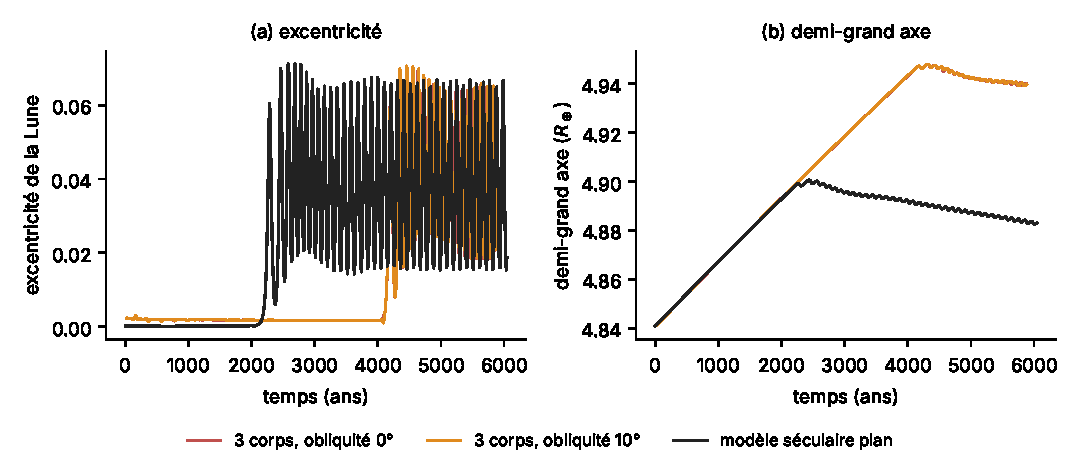
\includegraphics[width=0.95\textwidth]{figures/evection3.pdf}
\caption{Cas lent. Excentricité (a) et demi-grand axe (b) de la Lune, calcul à trois corps (moyenne glissante de 25 ans) et modèle séculaire plan. Les courbes à trois corps sont décalées dans le temps, la capture ayant lieu à un demi-grand axe un peu plus grand, mais leur amplitude est la même.\label{fig:evection3}}
\end{figure}

\begin{itemize}
\item \textbf{Balayage lent} (la résonance est traversée en plusieurs milliers d'années). La Lune est capturée dans la résonance en trois corps comme en séculaire, pour des obliquités de $0^\circ$ et de $10^\circ$ et pour trois intensités de marée lunaire. L'excentricité oscille entre environ $0{,}015$ et $0{,}07$ dans les deux modèles. Le taux de retrait est de $6{,}7\times10^{-4}\,\LEM$ par millier d'ans en trois corps contre $7{,}2\times10^{-4}$ en séculaire~: le trois corps donne \textbf{92 à 93\,\%} du taux séculaire.
\item La résonance est étroite (environ $0{,}3\,\%$ en demi-grand axe). La capture se produit à un demi-grand axe un peu plus grand en trois corps ($4{,}945\,\Rt$ contre $4{,}90\,\Rt$), d'où le décalage de la figure~\ref{fig:evection3}.
\item \textbf{Balayage rapide.} La capture est rare dans les deux modèles (excentricité maximale inférieure ou égale à $0{,}04$ dans les huit réalisations à trois corps). La capture dépend donc de la vitesse de balayage, et les deux modèles s'accordent sur ce point.
\end{itemize}

Les résultats du modèle séculaire sont donc reproduits en trois corps pour le balayage lent, avec un taux de retrait de 7 à 8\,\% plus faible. L'effet de cet écart sur les parts de fermeture est testé à l'annexe~\ref{app:ferm}. Le contrôle porte sur un nombre limité de cas~; il ne couvre pas toute la grille du tableau~\ref{tab:couple}.

\subsection{Durée de la capture}

Le retrait total est approximativement le taux de retrait multiplié par la durée pendant laquelle la Lune reste capturée~; la durée est donc une grandeur à connaître. Elle a été mesurée dans le modèle séculaire, pour $108$ trajectoires~: durée de contraction $\tau_c=2\times10^5$, $5\times10^5$ et $10^6$ ans, marée terrestre précoce de $0{,}03$, $0{,}1$ et $0{,}3\,\%$ de la référence, dissipation lunaire $(k_2/Q)_L=3\times10^{-4}$, $10^{-3}$ et $3\times10^{-3}$, et quatre phases d'arrivée dans la résonance. La capture est comptée tant que l'excentricité dépasse $0{,}02$ (pas de $500$ ans)~; $\Sigma$ est le moment cinétique retiré au système, en unités de $\LEM$.

\begin{table}[htbp]
\centering\footnotesize\setlength{\tabcolsep}{5pt}
\caption{Durée de capture (en milliers d'ans) et retrait cumulé $\Sigma$ (en $\LEM$), selon la durée de contraction $\tau_c$, la marée terrestre précoce (en \% de la référence) et la dissipation lunaire $(k_2/Q)_L$. Chaque case regroupe quatre phases d'arrivée~; on donne minimum / médiane / maximum.\label{tab:duree}}
\begin{tabular}{ccccc}\toprule
$\tau_c$ (ans) & marée précoce (\%) & $(k_2/Q)_L$ & durée (milliers d'ans) & $\Sigma$ ($\LEM$) \\\midrule
$2\times10^5$ & 0,03 & $3\times10^{-4}$ & 137 / 147 / 152 & 0,12 / 0,13 / 0,13\\
$2\times10^5$ & 0,03 & $10^{-3}$ & 42 / 47 / 50 & 0,07 / 0,07 / 0,07\\
$2\times10^5$ & 0,03 & $3\times10^{-3}$ & 7 / 8 / 10 & 0,03 / 0,03 / 0,03\\
$2\times10^5$ & 0,1 & $3\times10^{-4}$ & 2 / 3 / 4 & 0,00 / 0,00 / 0,00\\
$2\times10^5$ & 0,1 & $10^{-3}$ & 54 / 60 / 76 & 0,07 / 0,08 / 0,12\\
$2\times10^5$ & 0,1 & $3\times10^{-3}$ & 19 / 20 / 22 & 0,05 / 0,05 / 0,06\\
$2\times10^5$ & 0,3 & $3\times10^{-4}$ & 6 / 6 / 6 & 0,01 / 0,01 / 0,01\\
$2\times10^5$ & 0,3 & $10^{-3}$ & 0 / 0 / 0 & 0,00 / 0,00 / 0,00\\
$2\times10^5$ & 0,3 & $3\times10^{-3}$ & 0 / 8 / 20 & 0,00 / 0,03 / 0,06\\
\midrule
$5\times10^5$ & 0,03 & $3\times10^{-4}$ & 266 / 270 / 273 & 0,22 / 0,22 / 0,22\\
$5\times10^5$ & 0,03 & $10^{-3}$ & 98 / 102 / 106 & 0,13 / 0,13 / 0,13\\
$5\times10^5$ & 0,03 & $3\times10^{-3}$ & 14 / 15 / 20 & 0,06 / 0,06 / 0,06\\
$5\times10^5$ & 0,1 & $3\times10^{-4}$ & 4 / 130 / 264 & 0,00 / 0,12 / 0,25\\
$5\times10^5$ & 0,1 & $10^{-3}$ & 96 / 112 / 126 & 0,13 / 0,15 / 0,19\\
$5\times10^5$ & 0,1 & $3\times10^{-3}$ & 33 / 41 / 46 & 0,07 / 0,10 / 0,10\\
$5\times10^5$ & 0,3 & $3\times10^{-4}$ & 6 / 7 / 7 & 0,01 / 0,01 / 0,01\\
$5\times10^5$ & 0,3 & $10^{-3}$ & 0 / 45 / 91 & 0,00 / 0,10 / 0,21\\
$5\times10^5$ & 0,3 & $3\times10^{-3}$ & 0 / 12 / 24 & 0,00 / 0,04 / 0,09\\
\midrule
$10^6$ & 0,03 & $3\times10^{-4}$ & 414 / 420 / 434 & 0,30 / 0,30 / 0,30\\
$10^6$ & 0,03 & $10^{-3}$ & 158 / 164 / 170 & 0,19 / 0,19 / 0,19\\
$10^6$ & 0,03 & $3\times10^{-3}$ & 28 / 29 / 31 & 0,10 / 0,10 / 0,10\\
$10^6$ & 0,1 & $3\times10^{-4}$ & 4 / 4 / 4 & 0,00 / 0,00 / 0,00\\
$10^6$ & 0,1 & $10^{-3}$ & 146 / 162 / 178 & 0,18 / 0,20 / 0,26\\
$10^6$ & 0,1 & $3\times10^{-3}$ & 60 / 70 / 76 & 0,12 / 0,16 / 0,19\\
$10^6$ & 0,3 & $3\times10^{-4}$ & 6 / 7 / 8 & 0,01 / 0,01 / 0,01\\
$10^6$ & 0,3 & $10^{-3}$ & 0 / 56 / 117 & 0,00 / 0,13 / 0,27\\
$10^6$ & 0,3 & $3\times10^{-3}$ & 34 / 36 / 40 & 0,09 / 0,10 / 0,11\\
\bottomrule
\end{tabular}
\end{table}

\begin{figure}[htbp]
\centering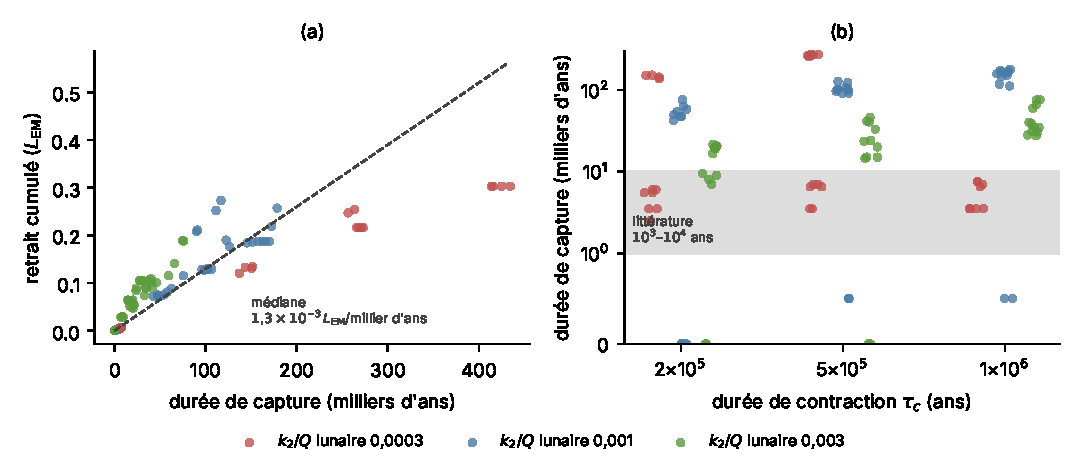
\includegraphics[width=\textwidth]{figures/duree_capture.pdf}
\caption{Durée de capture dans l'évection pour les $108$ trajectoires du tableau~\ref{tab:duree}. (a)~Retrait cumulé en fonction de la durée~; la droite en tirets est le taux médian. (b)~Durée en fonction de $\tau_c$~; la bande grise indique les passages de $10^3$ à $10^4$ ans que rapporte la littérature.\label{fig:duree}}
\end{figure}

\paragraph{Ce que montre la grille.}
\begin{itemize}
\item Sur $108$ trajectoires, $8$ ne sont pas capturées (excentricité maximale inférieure à $0{,}02$)~; toutes ont une marée précoce de $0{,}3\,\%$. Parmi les $100$ trajectoires capturées, la durée va de $0{,}5$ à $435$ milliers d'ans, avec une médiane de $39$ milliers d'ans (de $3{,}5$ au premier décile à $186$ au dernier). Au total, $38$ trajectoires sur $108$ ($35\,\%$) durent moins de $10^4$ ans, y compris les non-captures, et $56$ ($52\,\%$) durent $3\times10^4$ ans ou plus.
\item Le retrait est proportionnel à la durée~: pour les trajectoires capturées, il vaut en médiane $1{,}3\times10^{-3}\,\LEM$ par millier d'ans, du même ordre que le taux de l'annexe~\ref{app:evec}. Il atteint au plus $0{,}30\,\LEM$, et $0{,}10\,\LEM$ ou plus dans $44\,\%$ des trajectoires.
\item La durée dépend fortement de la marée précoce. Les médianes sont de $102$, $50$ et $6{,}5$ milliers d'ans pour $0{,}03$, $0{,}1$ et $0{,}3\,\%$~: plus la marée précoce est forte, plus la Lune sort vite de la résonance. Elle augmente aussi avec $\tau_c$ (médianes de $13$, $41$ et $50$ milliers d'ans), mais pas de façon monotone avec la dissipation lunaire~: c'est la combinaison des trois paramètres qui compte, comme le montre le tableau~\ref{tab:duree}.
\item L'excentricité maximale atteinte a pour médiane $0{,}066$ et pour maximum $0{,}19$.
\end{itemize}

\paragraph{Comparaison avec la littérature.}
Les passages dans l'évection que rapportent \citet{WardCanupRufu2020} et \citet{RufuCanup2020} durent de l'ordre de $10^3$ à $10^4$ ans et retirent de quelques pour cent à une dizaine de pour cent du moment cinétique~; \citet{Zahnle2015} obtiennent, pour une évolution lente, une capture quasi certaine mais une excentricité faible. Dans notre grille, la moitié des captures environ durent $3\times10^4$ ans ou plus, soit au moins trois fois la borne haute de ces passages, et elles retirent davantage. Ces durées dépendent de la marée précoce et de la dissipation lunaire, qui sont des paramètres posés (section~\ref{sec:couple}), non des résultats~: la comparaison indique ce que ces paramètres doivent valoir pour que la fermeture soit possible, elle ne les établit pas. Le calcul qui les fixerait est celui de la marée d'un corps mou, avec la viscosité de sa matière, inscrit au programme du tableau~\ref{tab:programme}.

\section{Fermeture du bilan~: sensibilité et états refondus}
\label{app:ferm}

Cette annexe prolonge la section~\ref{sec:couple}. Statut~: \stCalc. Les parts de trajectoires sont des parts de grille, non des probabilités~; une trajectoire pèse $2{,}8$ points de pourcentage.

\subsection{Sensibilité au rendement de l'évection}

L'annexe~\ref{app:trois} montre que le modèle trois corps donne $92$ à $93\,\%$ du taux de retrait du modèle séculaire. Pour savoir si un tel écart change les parts de fermeture, le retrait $\Sigma$ de chaque trajectoire de la grille du tableau~\ref{tab:couple} a été rescalé par $f=1$, $0{,}925$ et $0{,}85$ (36 trajectoires par $\Delta L_B$ et $\tau_c$).

\begin{table}[htbp]
\centering\footnotesize\setlength{\tabcolsep}{4pt}
\caption{Parts de fermeture (\%) pour $\varepsilon=0{,}03\,;0{,}05\,;0{,}08\,;0{,}10\,\LEM$ selon le rendement $f$ de l'évection.\label{tab:sensib}}
\begin{tabular}{ccccc}\toprule
$\tau_c$ (ans) & $\Delta L_B$ & $f=1$ & $f=0{,}925$ & $f=0{,}85$ \\\midrule
$3\times10^5$ & 0 & 17 19 33 39 & 6 17 28 33 & 3 14 25 33\\
 & 0,04 & 17 31 47 56 & 22 28 47 56 & 14 22 33 50\\
 & 0,07 & 8 36 44 56 & 11 19 44 56 & 11 17 42 56\\\midrule
$5\times10^5$ & 0 & 11 25 44 50 & 17 31 44 44 & 19 25 31 44\\
 & 0,04 & 6 31 50 75 & 11 39 47 64 & 19 25 44 56\\
 & 0,07 & 22 31 64 69 & 28 39 67 69 & 14 42 56 69\\\midrule
$10^6$ & 0 & 25 25 39 58 & 25 33 39 69 & 8 33 47 50\\
 & 0,04 & 22 25 50 56 & 19 28 47 56 & 22 31 44 64\\
 & 0,07 & 8 33 44 50 & 14 36 50 50 & 14 31 50 61\\\midrule
$2\times10^6$ & 0 & 6 28 50 64 & 8 39 58 67 & 19 33 56 64\\
 & 0,04 & 19 22 33 47 & 22 25 44 50 & 14 25 47 56\\
 & 0,07 & 19 19 31 31 & 19 25 31 42 & 22 25 42 42\\\bottomrule
\end{tabular}
\end{table}

Les parts restent dans la même gamme (typiquement $30$ à $70\,\%$ pour $\varepsilon\ge0{,}08$) et les variations d'une colonne à l'autre, de quelques trajectoires, sont du même ordre que le pas de la grille~; on n'y lit pas de dérive systématique. Un retrait de $0{,}04$ à $0{,}07\,\LEM$ par la planète~$B$ donne les parts les plus élevées pour $\tau_c=5\times10^5$~ans ($64$ à $75\,\%$ à $\varepsilon=0{,}08$--$0{,}10$).

\subsection{États refondus de la phase C}

Le bilan couplé a été refait avec quatre états initiaux issus de la phase~C refaite avec fusion au contact (annexe~\ref{app:phaseC}) et retenant une Lune~: rotation de $6{,}2$~h (graines 1 et 2) et de $6{,}4$~h (graines 0 et 1). Les paramètres de marée et de contraction sont ceux du tableau~\ref{tab:couple}, $\Delta L_B=0$, $288$ trajectoires.

\begin{table}[htbp]
\centering\footnotesize\setlength{\tabcolsep}{4pt}
\caption{Fermeture du bilan avec les états refondus de la phase~C. Parts (\%) pour $\varepsilon=0{,}03\,;0{,}05\,;0{,}08\,;0{,}10\,\LEM$.\label{tab:refondu}}
\begin{tabular}{cccc}\toprule état de départ & $\tau_c$ (ans) & part qui ferme (\%) & Lune perdue\\\midrule
6,2 h, graine 1 & $5\times10^5$ & 11 22 28 31 & 0\\ & $10^6$ & 6 22 36 36 & 0\\
6,2 h, graine 2 & $5\times10^5$ & 28 28 36 47 & 0\\ & $10^6$ & 22 36 47 56 & 2\\
6,4 h, graine 0 & $5\times10^5$ & 22 25 47 67 & 0\\ & $10^6$ & 11 36 50 56 & 2\\
6,4 h, graine 1 & $5\times10^5$ & 19 25 44 64 & 0\\ & $10^6$ & 19 31 50 56 & 4\\\bottomrule\end{tabular}
\end{table}

Pour $\varepsilon=0{,}08$--$0{,}10$, les parts vont de $28$ à $67\,\%$ selon l'état, dans la gamme obtenue avec l'état du tableau~\ref{tab:couple} ($39$ à $58\,\%$ à $\Delta L_B=0$). Les quatre états refondus ferment donc le bilan sans que l'état de départ ait été choisi pour cela~; ils ne le font pas au même niveau, et l'écart entre états est du même ordre que l'écart entre graines de la phase~C.


\section{Phase C~: vitesses de collision, rotation initiale et seuils de fusion}
\label{app:phaseC}

Cette annexe prolonge la section~\ref{sec:methode} (règle de pâte, $H4$). Statut~: \stCalc, avec de petits échantillons que le texte signale. La phase~C est chaotique~: une même graine rejouée peut donner un résultat différent (la masse du corps dominant passe de $0{,}12$ à $0{,}41$ masse lunaire pour $6{,}0$~h et la graine~0), si bien qu'une réalisation isolée ne permet pas de conclure.

\subsection{Distribution des vitesses de collision}

Dans quatre réalisations à $6{,}0$~h, la vitesse relative de chacune des $768$ collisions a été enregistrée. La médiane est de $2{,}3$~km\,s$^{-1}$~; les quartiles sont $1{,}4$ et $3{,}5$~km\,s$^{-1}$, $10\,\%$ des collisions sont sous $0{,}9$ et $10\,\%$ au-dessus de $4{,}7$~km\,s$^{-1}$. Les parts sous un seuil sont $3\,\%$ ($0{,}5$), $13\,\%$ ($1$), $43\,\%$ ($2$) et $66\,\%$ ($3$~km\,s$^{-1}$). Seules $5{,}7\,\%$ des collisions sont plus lentes que la vitesse d'évasion du couple qui se heurte~; elles se concentrent dans les trente premiers jours.

\begin{figure}[htbp]
\centering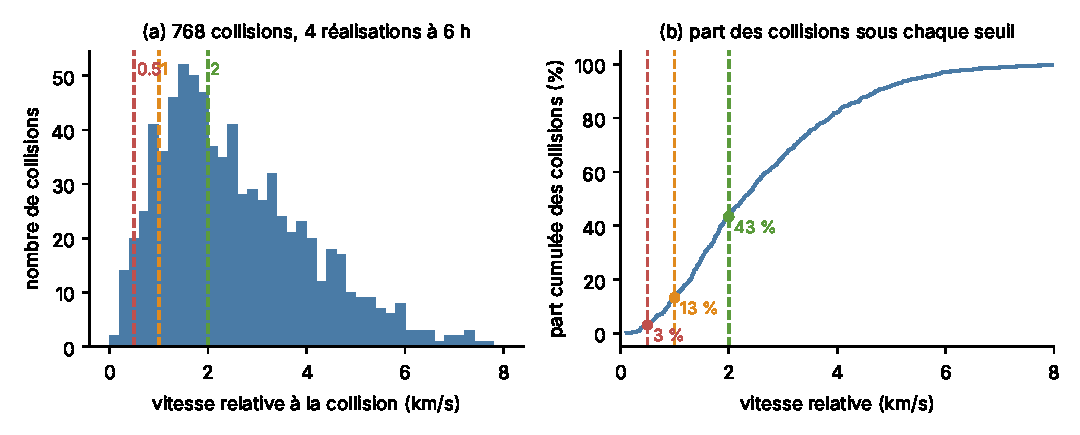
\includegraphics[width=0.95\linewidth]{vrel.pdf}
\caption{Vitesses relatives des $768$ collisions (phase~C, $6{,}0$~h, quatre réalisations)~: histogramme (a) et part cumulée sous chaque seuil (b).}
\end{figure}

\subsection{Balayage de la rotation initiale}

\begin{table}[htbp]
\centering\small
\caption{Phase~C avec fusion au contact (OMB $=90^\circ$), une à trois réalisations par rotation. Le verdict suit la règle de la section~\ref{sec:methode}. Les lignes «~contrôle~» sont des rejeux instrumentés (vitesses de collision enregistrées).\label{tab:rotscan}}
\begin{tabular}{cccccc}\toprule rotation & graine & $M_1$ ($\ML$) & $a_1$ ($\Rt$) & $e_1$ & verdict\\\midrule
6,0 h & 0 & 0,12 & 3,11 & 0,33 & n'aboutit pas\\
6,0 h & 0 (contrôle) & 0,41 & 4,55 & 0,15 & n'aboutit pas\\
6,0 h & 1 (contrôle) & 0,95 & 3,38 & 0,11 & retenu\\
6,2 h & 0 & 0,14 & 2,91 & 0,17 & n'aboutit pas\\
6,2 h & 1 & 0,91 & 3,13 & 0,15 & retenu\\
6,2 h & 2 & 0,95 & 3,02 & 0,14 & retenu\\
6,4 h & 0 & 1,02 & 2,79 & 0,04 & retenu\\
6,4 h & 1 & 1,02 & 3,28 & 0,13 & retenu\\
6,8 h & 0 & 0,37 & 4,94 & 0,29 & n'aboutit pas\\
6,8 h & 1 & 1,09 & 3,09 & 0,10 & retenu\\\bottomrule\end{tabular}
\end{table}

Six réalisations sur dix donnent une Lune retenue, de $0{,}91$ à $1{,}09$ masse lunaire. Pour une même rotation, deux graines peuvent donner des verdicts différents~; avec un à trois tirages par valeur, rien ne permet de dire que la rotation décide du verdict. Deux autres contrôles à $6{,}0$~h, interrompus à $320$ et $85$ jours, ne sont pas comptés.

\subsection{Seuils de fusion}

L'hypothèse $H4$ (fusion au contact) a été remplacée par une loi à seuil~: deux corps fusionnent si leur vitesse relative est inférieure à $v_{\rm crit}$, et rebondissent sinon (coefficient de restitution $0{,}3$). La grille compare $v_{\rm crit}=0{,}5\,;1\,;2$~km\,s$^{-1}$ sur quatre états qui retiennent une Lune avec fusion au contact (rotations $6{,}2$~h, graines 1 et 2, et $6{,}4$~h, graines 0 et 1)~: douze simulations de $150$ jours, comparées à la fusion au contact des mêmes graines au même instant.

\begin{table}[htbp]
\centering\small\setlength{\tabcolsep}{4pt}
\caption{Masse $M_1$ du corps dominant (en $\ML$) à $150$ jours selon le seuil de fusion~; en gras, les cas qui satisfont le critère de Lune retenue ($M_1>0{,}5$ et $a_1\ge R_{\rm co}$).\label{tab:seuils}}
\begin{tabular}{lccccc}\toprule $v_{\rm crit}$ & 6,2 h g.\,1 & 6,4 h g.\,0 & 6,2 h g.\,2 & 6,4 h g.\,1 & Lunes retenues\\\midrule
contact & \textbf{0,89} & \textbf{1,00} & \textbf{0,91} & \textbf{1,02} & 4 sur 4\\
2 km\,s$^{-1}$ & \textbf{0,73} & 0,17 & \textbf{0,65} & \textbf{0,68} & 3 sur 4\\
1 km\,s$^{-1}$ & 0,46 & \textbf{0,52} & 0,39 & 0,37 & 1 sur 4\\
0,5 km\,s$^{-1}$ & 0,12 & 0,20 & 0,13 & 0,21 & 0 sur 4\\\bottomrule\end{tabular}
\end{table}

\begin{figure}[htbp]
\centering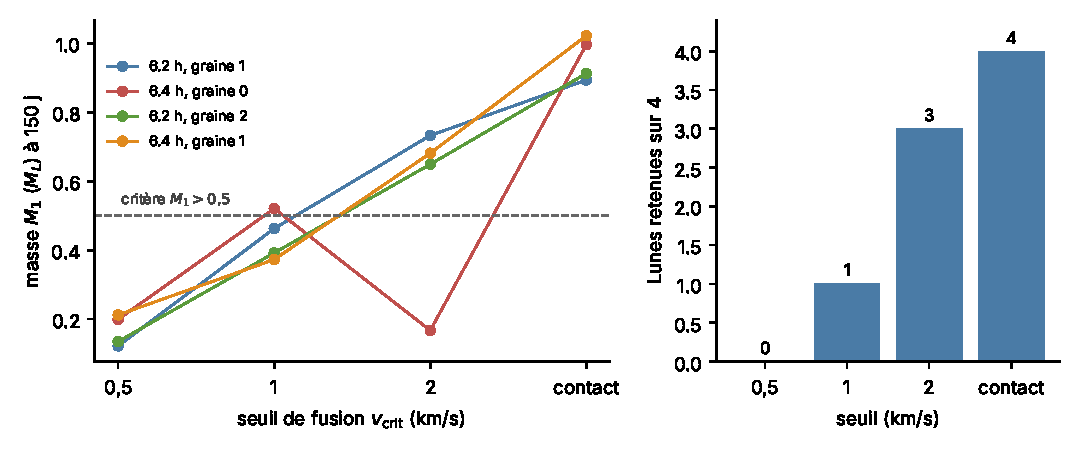
\includegraphics[width=0.95\linewidth]{seuils.pdf}
\caption{Masse du corps dominant (a) et nombre de Lunes retenues (b) selon le seuil de fusion, pour les quatre états.}
\end{figure}

Dans cet échantillon, la masse retenue augmente nettement quand le seuil passe de $0{,}5$ à $2$~km\,s$^{-1}$, avec une exception (rotation $6{,}4$~h, graine~0, où le seuil de $2$~km\,s$^{-1}$ disperse la Lune à $a_1=7{,}9\,\Rt$). Une Lune est retenue dans trois états sur quatre avec un seuil de $2$~km\,s$^{-1}$, dans un sur quatre à $1$ et dans aucun à $0{,}5$. La formation d'une Lune demande donc ici une accrétion efficace jusqu'à environ $2$~km\,s$^{-1}$~; elle ne demande pas la fusion à toute vitesse~: avec un seuil de $2$~km\,s$^{-1}$, plus de la moitié des collisions ($57\,\%$) rebondissent, et la Lune est tout de même retenue dans trois cas sur quatre.

\subsection{Limites}

Une seule simulation par case~; $150$ jours seulement (la structure se fixe dans les premiers mois, ce que nous n'avons pas vérifié pour chaque état à $365$ jours)~; coefficient de restitution fixé à $0{,}3$ et non testé~; seuil porté par la seule vitesse relative, sans dépendance en température. Les essais préliminaires à $6{,}0$~h, un tirage par seuil, n'aboutissaient pas~; $6{,}0$~h est aussi la rotation la plus incertaine avec la fusion au contact (tableau~\ref{tab:rotscan}). La carte vitesse--température de l'accrétion reste à tracer~: elle demande une loi de collision qui dépend de la température, que le code ne contient pas. Les sorties complètes sont dans le paquet décrit à l'annexe~\ref{app:repro}.



\section{Glossaire}

\begin{description}[leftmargin=3.2cm,style=nextline,itemsep=2pt]
\item[Obliquité] angle entre l'axe de rotation d'une planète et la normale à son orbite.
\item[Planète~$B$] la seconde planète rocheuse (de $0{,}95$ masse terrestre) dont le survol, par gravitation seule, redistribue le disque.
\item[Proto-Terre] la Terre avant la formation de la Lune~: chaude, molle, gonflée.
\item[Corps mou] matière pâteuse, ni liquide ni solide froid, dont la déformation sous la marée dissipe de l'énergie.
\item[Limite de Roche] distance en deçà de laquelle la marée de la planète déchire un corps fluide.
\item[Rayon de corotation] distance à laquelle un corps orbite aussi vite que la Terre tourne~; au-delà, la marée repousse le corps, en deçà elle l'attire.
\item[Rétrograde] à contresens de la rotation de la Terre.
\item[Phases A, B, C] existence du disque (A), survol (B), assemblage et évolution (C).
\item[$\LEM$] moment cinétique du système Terre--Lune actuel, $3{,}5\times10^{34}$~kg\,m$^2$\,s$^{-1}$.
\item[$k_2/Q$] mesure de la dissipation de marée d'un corps~: plus elle est grande, plus le corps transforme la marée en chaleur.
\item[Évection] résonance entre la précession du périgée du satellite et le mouvement apparent du Soleil, qui retire du moment cinétique au système.
\item[Séculaire] qualifie un calcul qui moyenne les mouvements rapides pour suivre l'évolution lente.
\end{description}

\bibliographystyle{unsrtnat}
\bibliography{refs}


\end{document}
